\documentclass[10pt,a4paper]{article}

\usepackage[utf8]{inputenc}
\usepackage[T1]{fontenc}
\usepackage[brazil]{babel}
\usepackage{amsmath,amssymb}
\usepackage{graphicx}
\usepackage[colorlinks=true,linkcolor=blue,citecolor=blue,urlcolor=blue]{hyperref}
\usepackage{float}
\usepackage{subcaption}
\usepackage{booktabs}
\usepackage{geometry}
\usepackage{xcolor}
\usepackage{titlesec}

\geometry{top=1.8cm, bottom=1.8cm, left=2cm, right=2cm}
\setlength{\parskip}{2pt}
\setlength{\parindent}{0pt}
\setlength{\abovecaptionskip}{4pt}
\setlength{\belowcaptionskip}{2pt}
\titlespacing{\section}{0pt}{8pt}{4pt}
\titlespacing{\subsection}{0pt}{6pt}{2pt}

\renewcommand{\figurename}{Figura}

\title{Projeto 03: Redes Neurais do zero com interpretabilidade\\ \large Breast Cancer Winsconsin (Diagnostic)}
\author{
  \small
  Rodrigo Banin Ferraz de Camargo (238257)
  \textbullet{}
    Caio Lima Albulquerque (288808) \\ \small Ricardo Andrade Oliveira Bello (247326)
  \date{\small\today}
}
\begin{document}

\maketitle

\section{Descrição da Implementação}
Este projeto trata do desenvolvimento de um modelo de Rede Neural (MLP) de classificação binária a partir do conjunto de dados \textit{Breast Cancer Wisconsin (Diagnostic)}, analisando-se a importância das \textit{features} e discutindo-se as decisões feitas pelo modelo com base nas entradas. 

A arquitetura da MLP foi implementada integralmente do zero utilizando apenas a biblioteca NumPy, com toda a lógica encapsulada na classe \texttt{MLP}. O fluxo do modelo contempla os seguintes componentes:

\begin{itemize}
    \item \textbf{Forward pass:} São feitos cálculos vetorizados camada a camada ($Z^{(l)} = A^{(l-1)} W^{(l)} + b^{(l)}$), utilizando-se a função de ativação ReLU nas camadas ocultas e Softmax na camada de saída. Para garantir estabilidade numérica e evitar \textit{overflow}, a implementação do Softmax subtrai o valor máximo de cada projeção antes da exponenciação ($Z_{est\acute{a}vel} = Z - \max(Z)$).
    
    \item \textbf{Backpropagation:} Realizam-se cálculos exatos dos gradientes a partir da camada de saída ($\frac{\partial L}{\partial Z^{(L)}} = \text{softmax}(Z^{(L)}) - y_{\text{one-hot}}$), propagando o erro para as matrizes de pesos das camadas anteriores por meio da regra da cadeia e da derivada da ReLU. O \textit{one-hot encoding} do alvo é tratado internamente.
    
    \item \textbf{Otimização:} O treinamento utiliza \textbf{Mini-Batch Gradient Descent}. Como funcionalidade extra, foi incorporada a atualização com momentum ($v \leftarrow \beta v - \alpha \frac{\partial L}{\partial W}$, $W \leftarrow W + v$) para acelerar a convergência e atenuar oscilações.
    
    \item \textbf{Inicialização e Função de Custo:} Os pesos adotam a inicialização avançada de He ($W \sim \mathcal{N}(0, \sqrt{2 / \text{fan\_in}})$) -- ideal para redes com ativação ReLU -- enquanto os vieses são inicializados em zero. A função de custo otimizada é a \textbf{Cross-Entropy} categórica ($L = -\frac{1}{N} \sum_{i=1}^{N} \log(\hat{y}_{i, y_i})$).
\end{itemize}

A arquitetura base utilizada para a maior parte dos experimentos possui a configuração \texttt{[30, 64, 32, 2]} (30 entradas correspondentes às features do \textit{dataset}, 64 e 32 neurônios nas camadas ocultas, e 2 saídas para as classes benigno/maligno). Além dos métodos de treino (\texttt{train}) e predição (\texttt{predict}), a classe integra de forma nativa os três algoritmos de interpretabilidade aplicados neste estudo: mapas de saliência, perturbação e ablação, calculados diretamente sobre os tensores da rede.

\section{Análise Exploratória de Dados}
O conjunto de dados utilizados é composto por 569 instâncias e 30 atributos numéricos contínuos. Esses atributos são derivados da análise de imagens digitais de Aspiração por Agulha Fina (FNA) de massas mamárias. Eles descrevem características geométricas, topológicas e de textura dos núcleos celulares, computadas em três variantes para cada imagem: média, erro padrão e o "pior" valor (média dos três maiores valores). 

A distribuição das classes apresenta um leve desbalanceamento, consistindo em 357 casos Benignos (62,7\%) e 212 Malignos (37,3\%), conforme ilustrado na Figura 1(a). Essa observação é fundamental, pois justifica a necessidade de utilizar um particionamento estratificado (\textit{stratified split}) para separar os conjuntos de treino e teste posteriormente, garantindo a representatividade das classes. Além disso, é importante destacar que como os atributos originais operam em ordens de grandeza muito distintas (\textit{e.g.} a área pode ultrapassar $2000$, enquanto a suavidade opera na casa de $0.01$), todos os dados foram submetidos a uma padronização estatística (\textit{z-score}) antes de alimentar o modelo. A Figura 1(b) ilustra a dispersão das variáveis após a normalização (média 0 e desvio padrão 1), crucial para evitar que a MLP priorize pesos de \textit{features} com maior magnitude absoluta durante o cálculo dos gradientes.

\begin{figure}[H]
    \centering
    \begin{subfigure}{0.33\textwidth}
        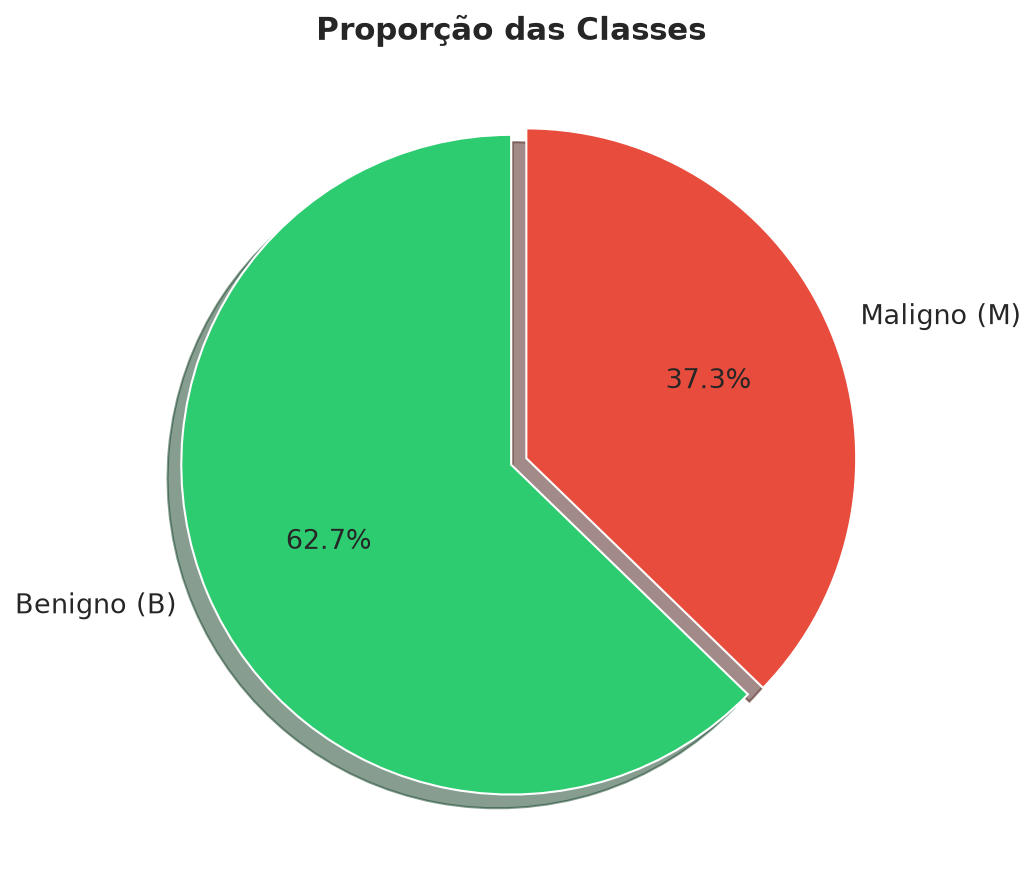
\includegraphics[width=\textwidth]{../images/01_distribuicao_classes.png}
        \caption{Distribuição das classes.}
    \end{subfigure}
    \hfill
    \begin{subfigure}{0.64\textwidth}
        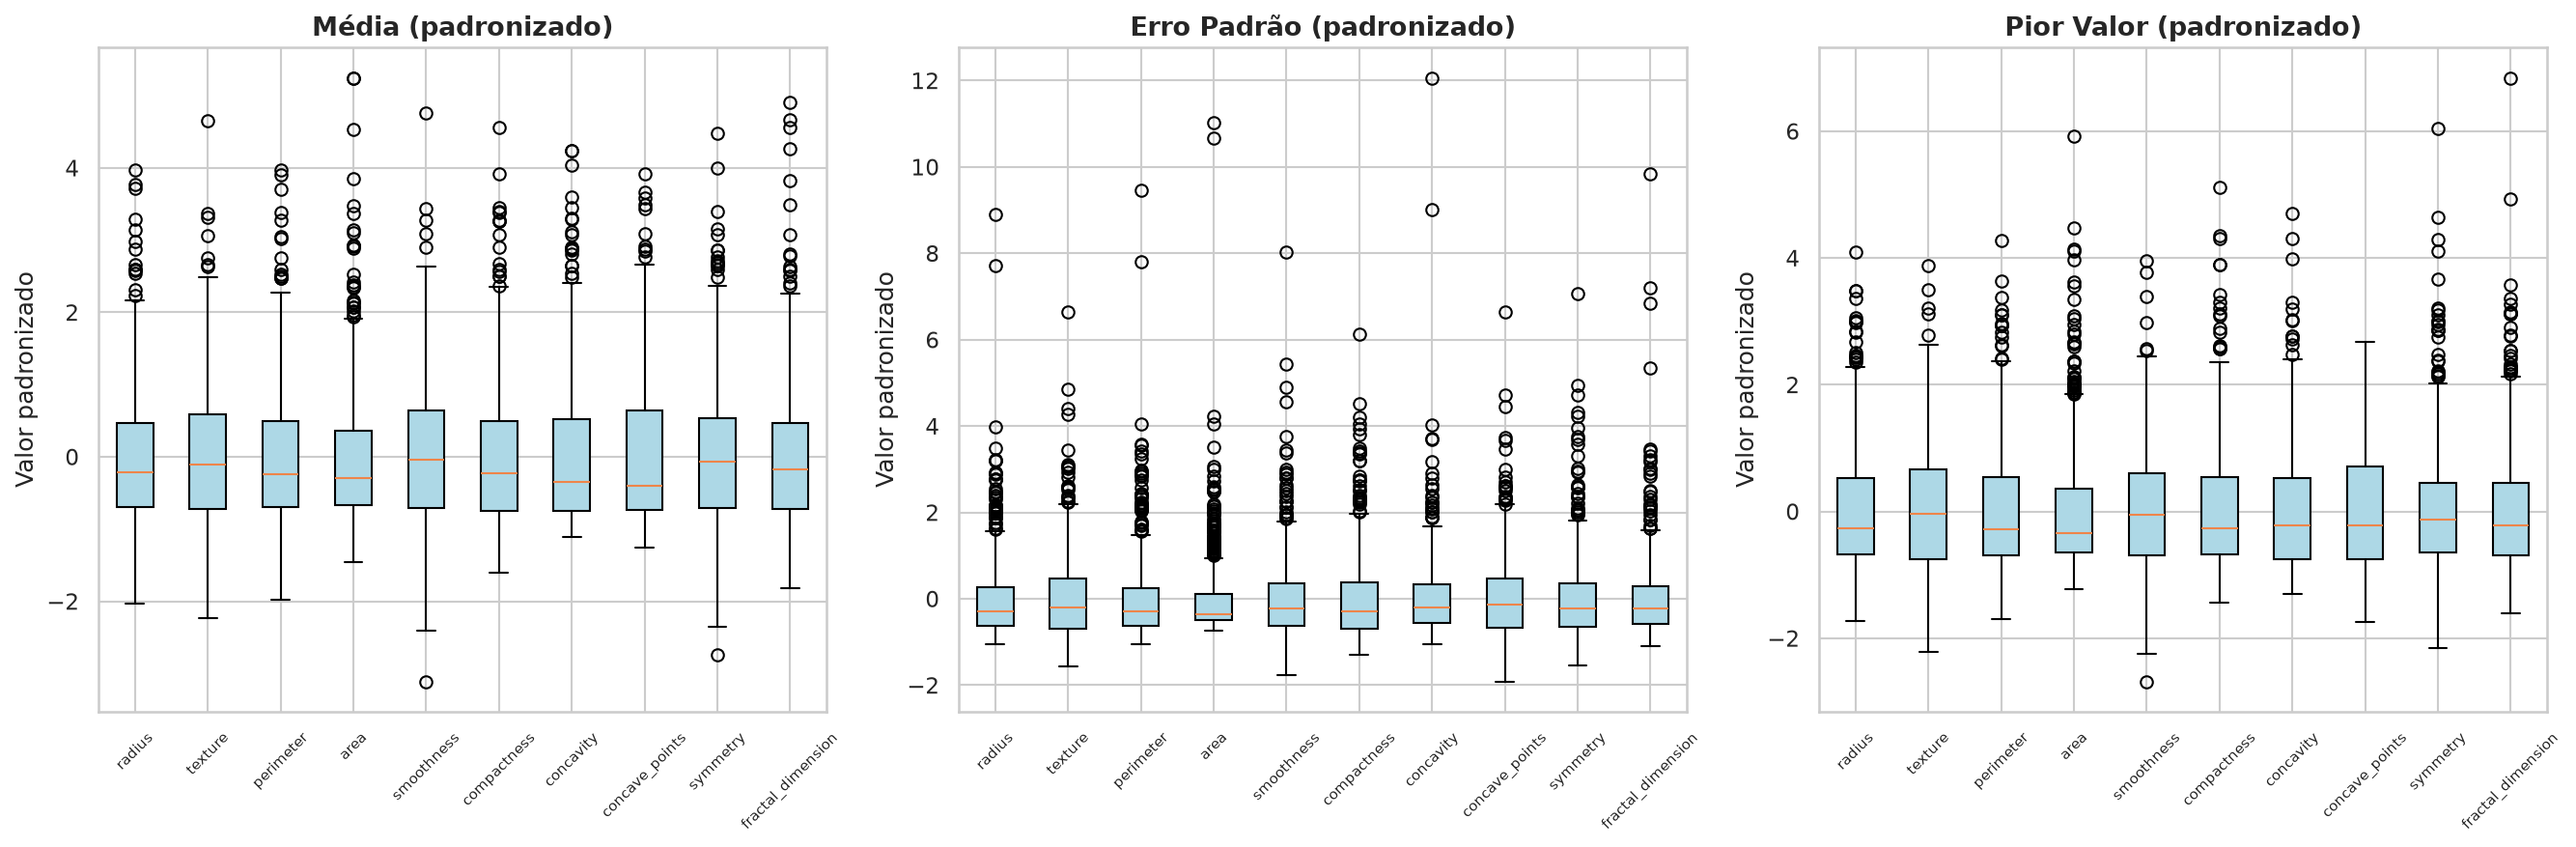
\includegraphics[width=\textwidth]{../images/02_boxplots_grupos.png}
        \caption{Boxplots padronizados por grupo (média, erro padrão, pior valor).}
    \end{subfigure}
\end{figure}

A análise das distribuições por meio de histogramas (Figura 2) revela que algumas características possuem um alto poder discriminativo de forma isolada. Atributos como \texttt{concave\_points}, \texttt{perimeter} e \texttt{area} mostram uma clara separação espacial entre instâncias benignas e malignas, onde valores mais elevados estão fortemente associados à tumores malignos. 

\begin{figure}[H]
    \centering
    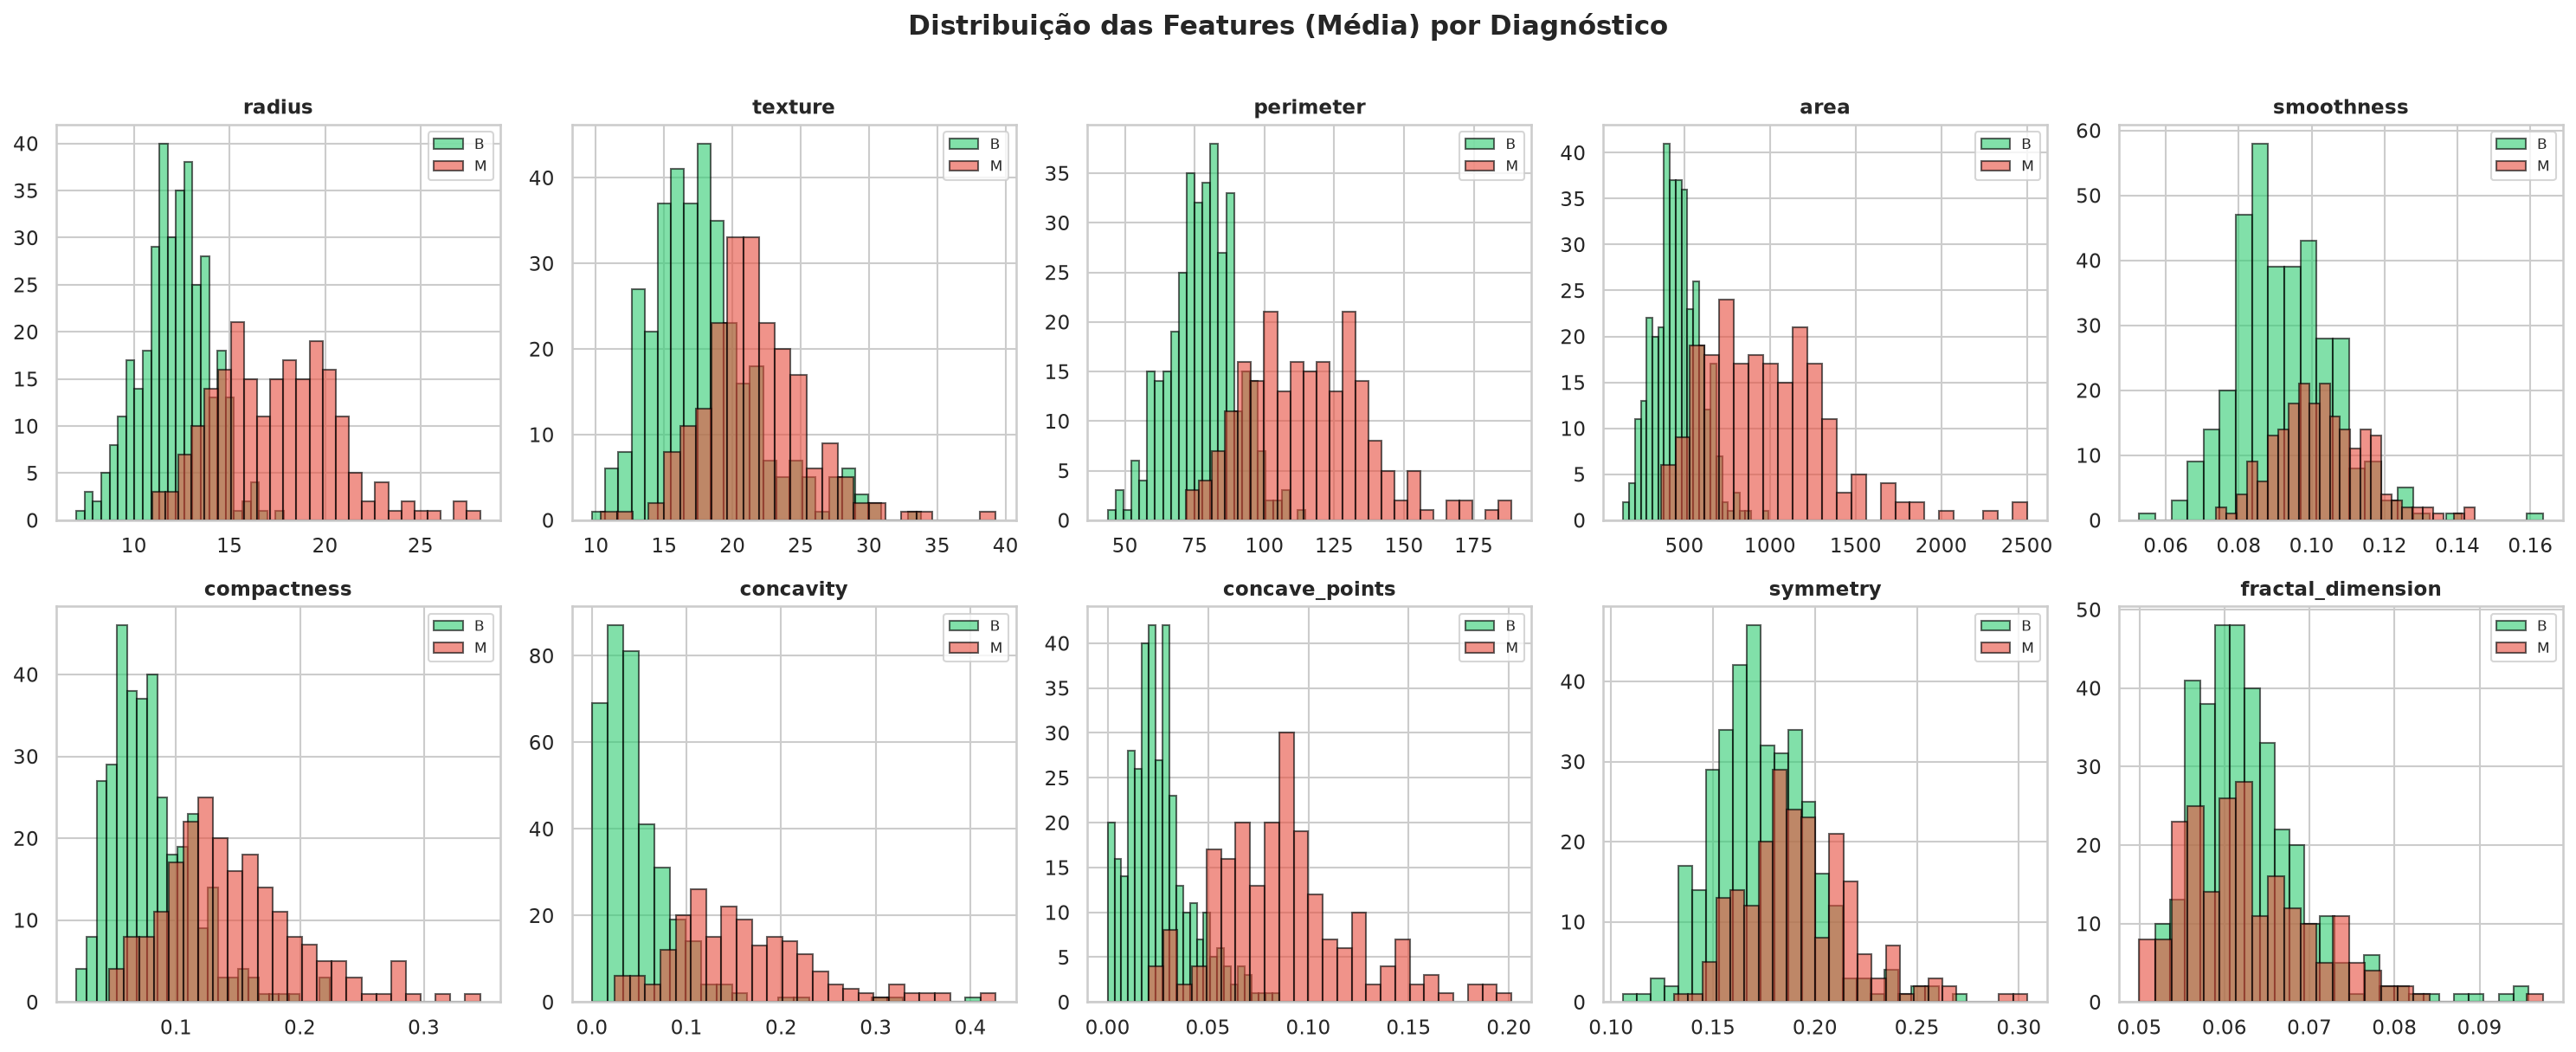
\includegraphics[width=0.85\textwidth]{../images/03_histogramas_mean.png}
    \caption{Distribuição das features de média por classe. \texttt{concave\_points}, \texttt{perimeter} e \texttt{area} mostram clara separação entre benignos (verde) e malignos (vermelho).}
\end{figure}

O \textit{pairplot} (Figura 3b) reitera que a combinação das \textit{features} mais discriminativas forma agrupamentos bem definidos, indicando que um modelo não linear como a MLP terá capacidade robusta para modelar a fronteira de decisão. Adicionalmente, a matriz de correlação (Figura 3a) evidencia alta multicolinearidade entre variáveis estritamente geométricas, como raio, perímetro e área, que apresentam correlação de Pearson quase perfeita ($r > 0.95$). 

\begin{figure}[H]
    \centering
    \begin{subfigure}{0.48\textwidth}
        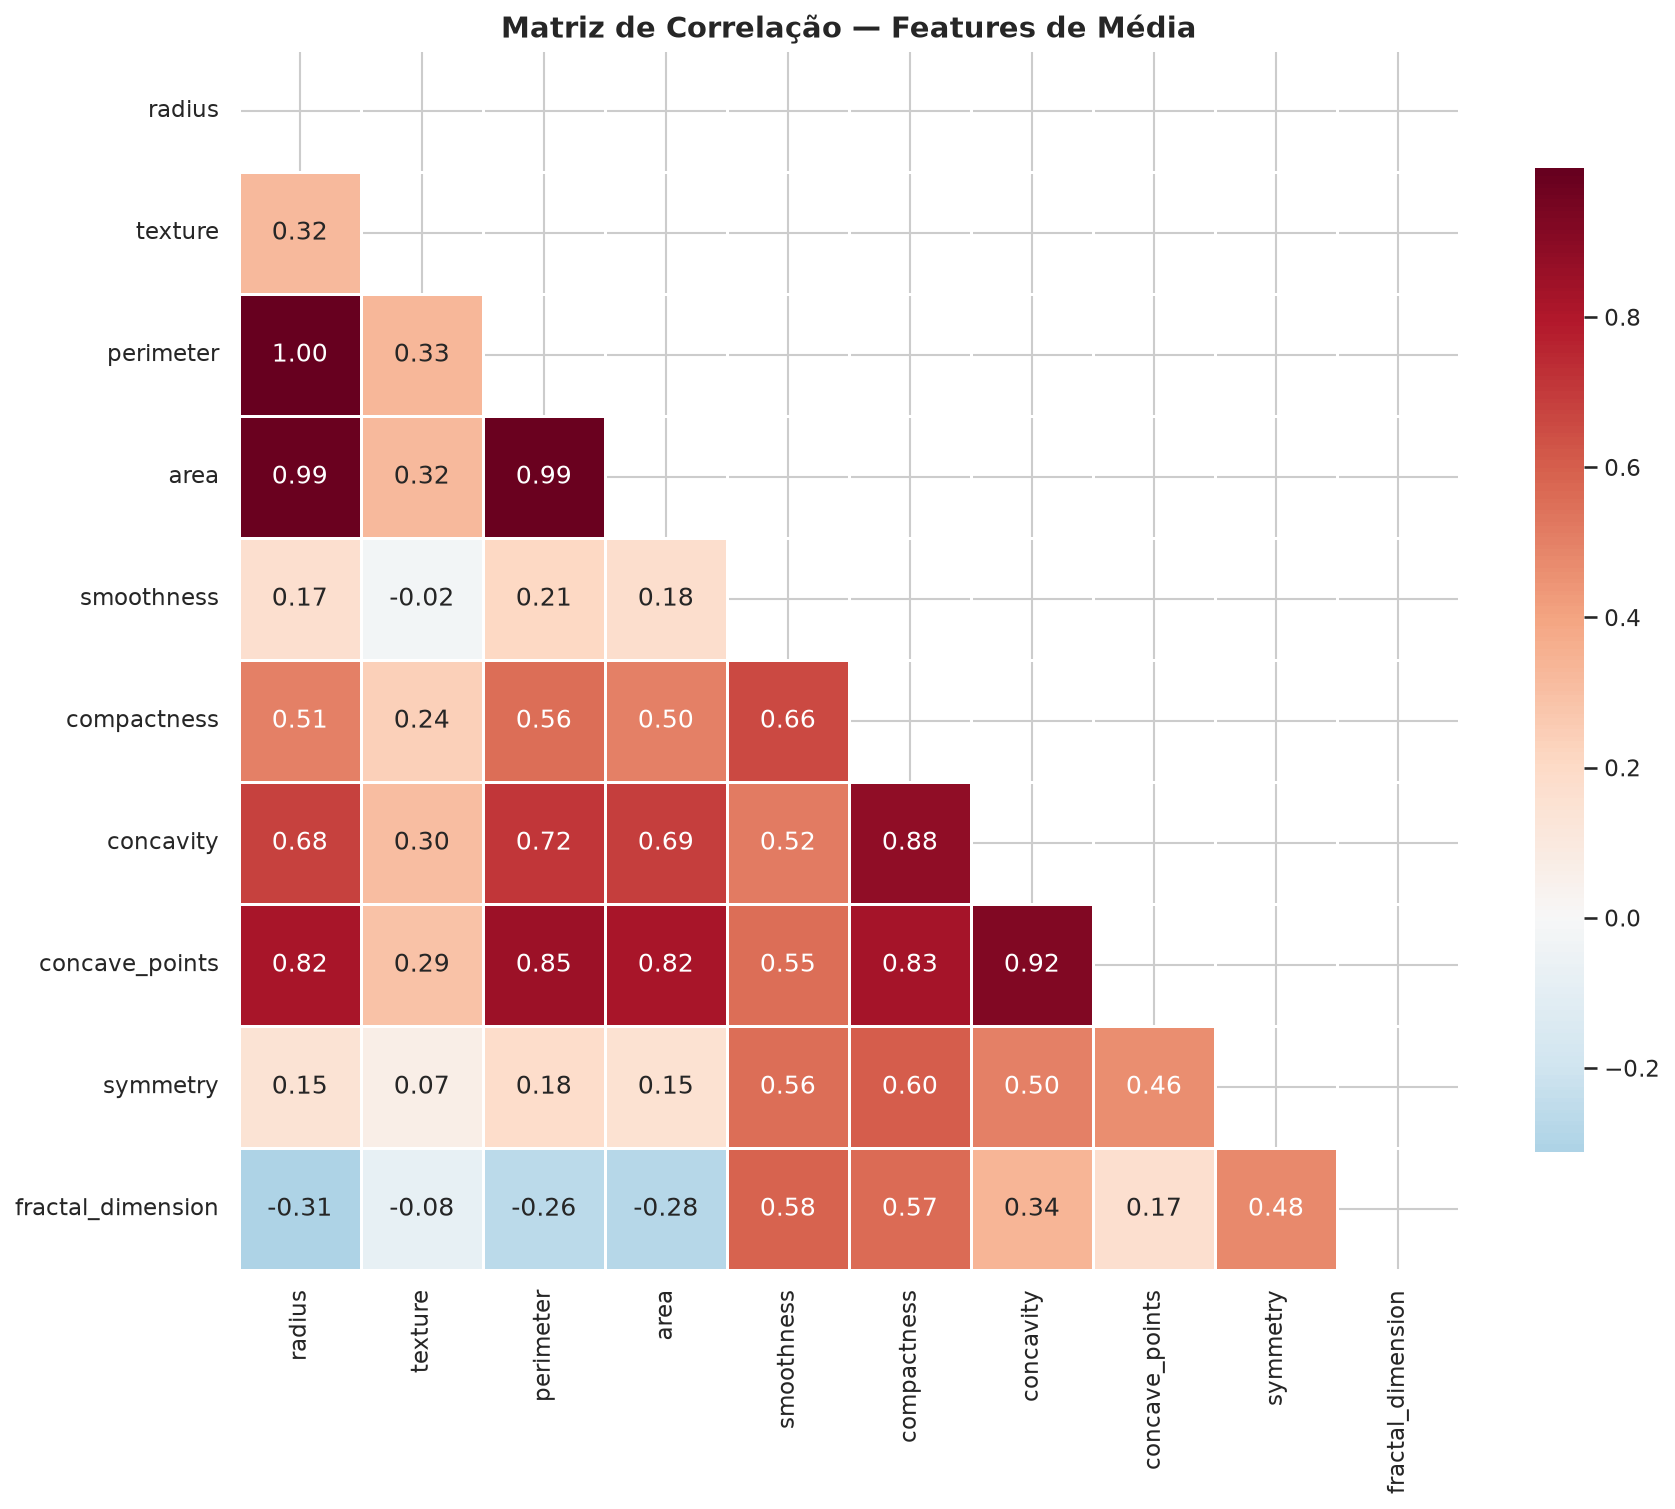
\includegraphics[width=\textwidth]{../images/04_correlacao_mean.png}
        \caption{Correlação das features de média. \texttt{radius}, \texttt{perimeter} e \texttt{area} são altamente correlacionados ($r>0{,}95$).}
    \end{subfigure}
    \hfill
    \begin{subfigure}{0.48\textwidth}
        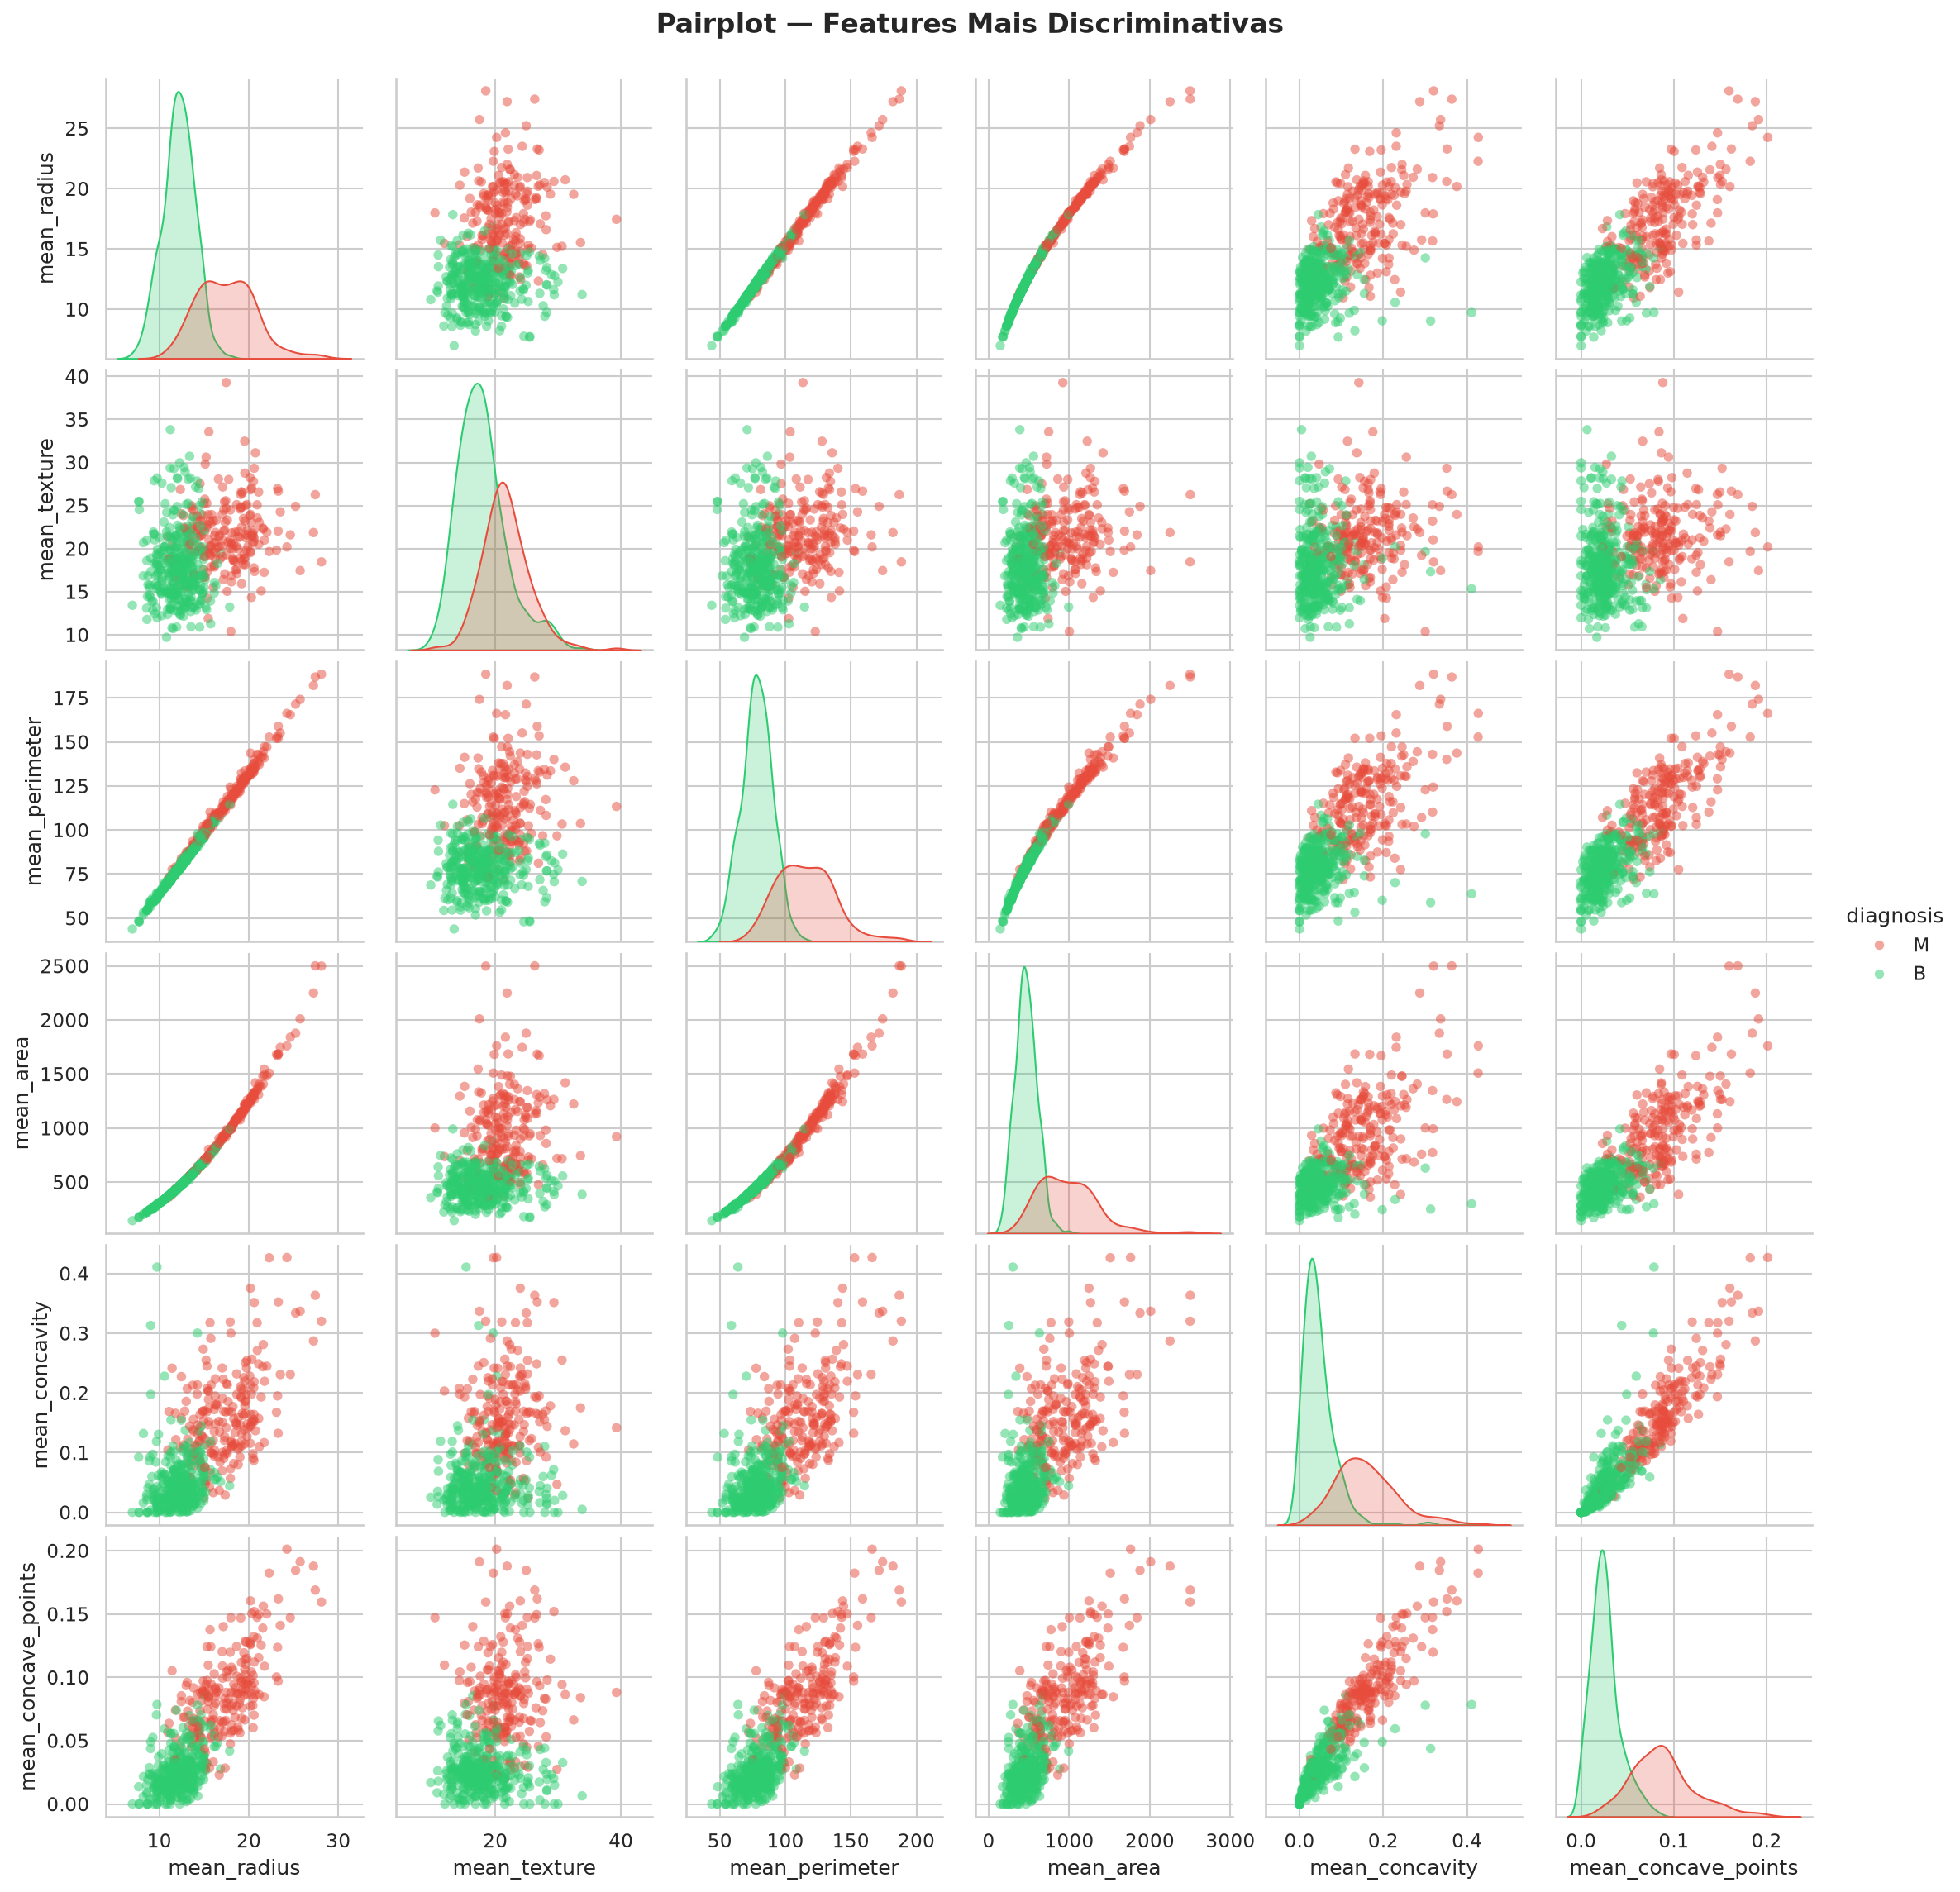
\includegraphics[width=\textwidth]{../images/05_pairplot.png}
        \caption{Pairplot das 6 features mais discriminativas.}
    \end{subfigure}
\end{figure}

\section{Treinamento e Avaliação}

Para a avaliação do desempenho do modelo implementado, o conjunto de dados original foi particionado na proporção clássica de $80\%$ para o conjunto de treinamento (455 instâncias) e $20\%$ para o conjunto de teste (114 instâncias). Adotou-se explicitamente um critério de \textit{stratified split} com o objetivo de preservar a proporção exata entre as classes benigna e maligna em ambos os subconjuntos, mitigando quaisquer distorções analíticas decorrentes do desbalanceamento original do \textit{dataset}. 

O modelo base para a consolidação das métricas foi estabelecido com a arquitetura \texttt{[30, 64, 32, 2]} (utilizando duas camadas ocultas), \textit{learning rate} estável $\alpha=0.01$, tamanho de mini-batch fixado em 32, e um horizonte de treinamento composto por 200 épocas. Os resultados estatísticos obtidos após a convergência dos pesos estão sumarizados na Tabela 1, disposta em paralelo ao comportamento histórico das curvas de aprendizado.

\begin{table}[H]
    \centering
    \begin{tabular}{lcc}
        \toprule
        Métrica & Treino & Teste \\
        \midrule
        Loss      & 0.0265 & 0.1027 \\
        Acurácia  & 0.9956 & \textbf{0.9825} \\
        \bottomrule
    \end{tabular}
    \quad
    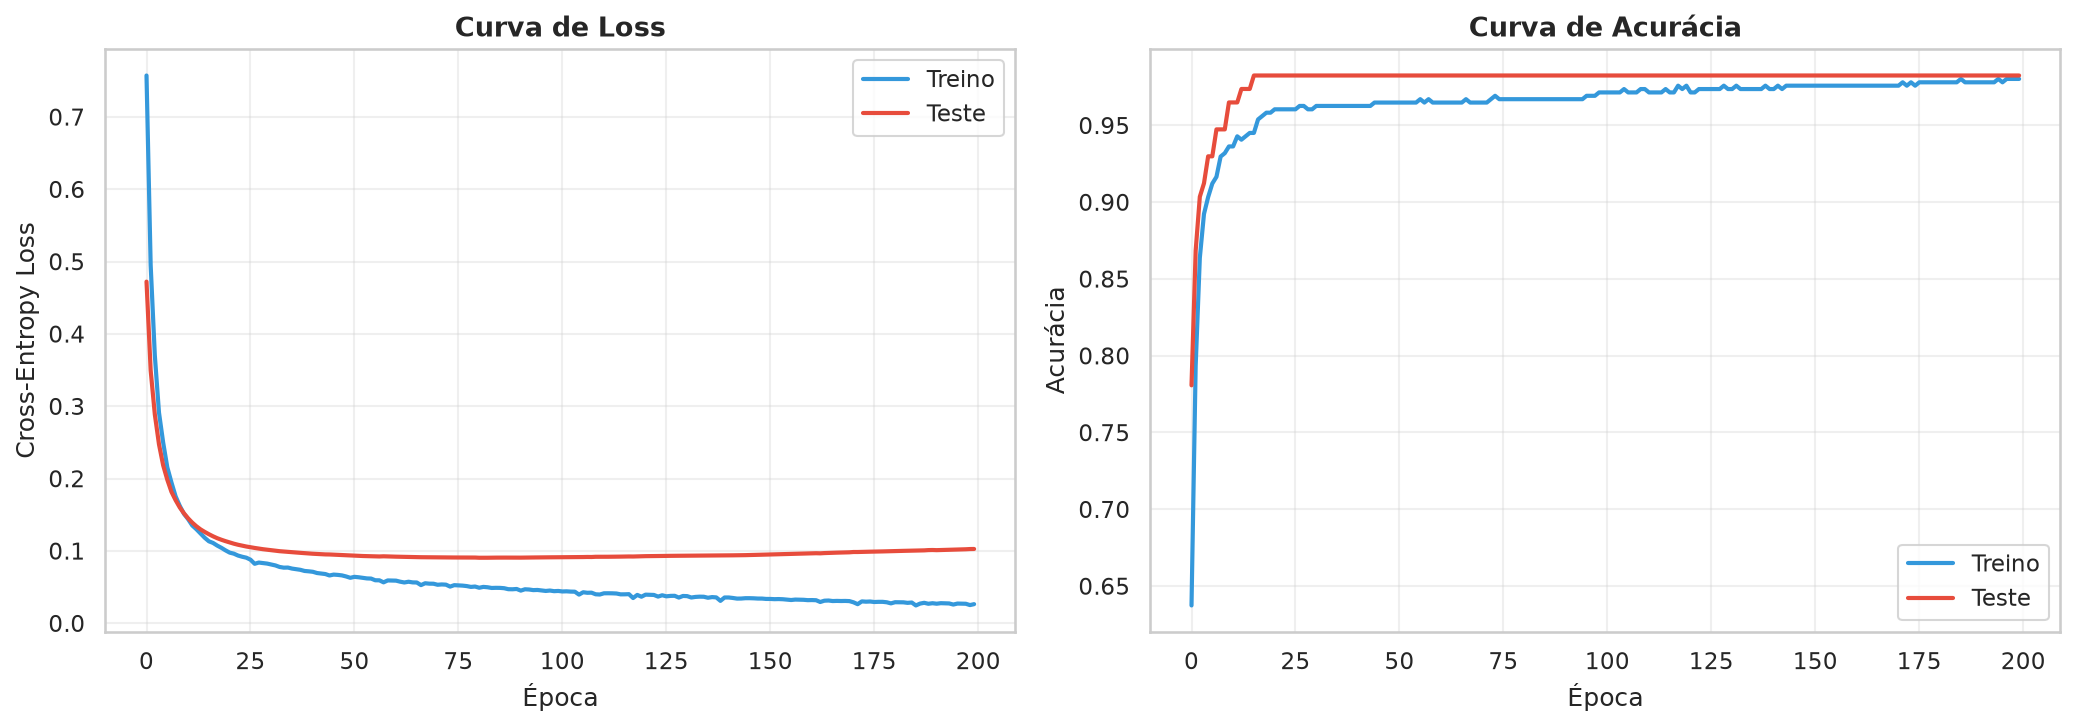
\includegraphics[width=0.55\textwidth]{../images/06_curvas_treinamento.png}
\end{table}

A partir do treinamento executado do zero, observa-se que o classificador linear atingiu uma acurácia notável de $98.25\%$ no conjunto de teste. A análise detalhada das curvas de treinamento revela importantes dinâmicas de otimização. Constata-se a ocorrência de um leve cenário de \textit{overfitting} a partir da época $\sim 40$, evidenciado pelo comportamento divergente das curvas de custo: enquanto a \textit{loss} de treino decai de forma contínua em direção a zero, a \textit{loss} de teste apresenta uma sutil inflexão ascendente. No entanto, esse início de memorização de ruído não resultou em prejuízos práticos para o modelo, visto que a curva de acurácia do conjunto de teste estabilizou-se de forma plana e resiliente até o final do processo, validando a robustez dos parâmetros aprendidos.

\subsection{Impacto dos Hiperparâmetros}

A flexibilidade do modelo desenvolvido permitiu mapear o comportamento da rede neural sob diferentes configurações operacionais. Os resultados empíricos desse mapeamento sistemático estão ilustrados na Figura 4.

\begin{figure}[H]
    \centering
    \begin{subfigure}{0.48\textwidth}
        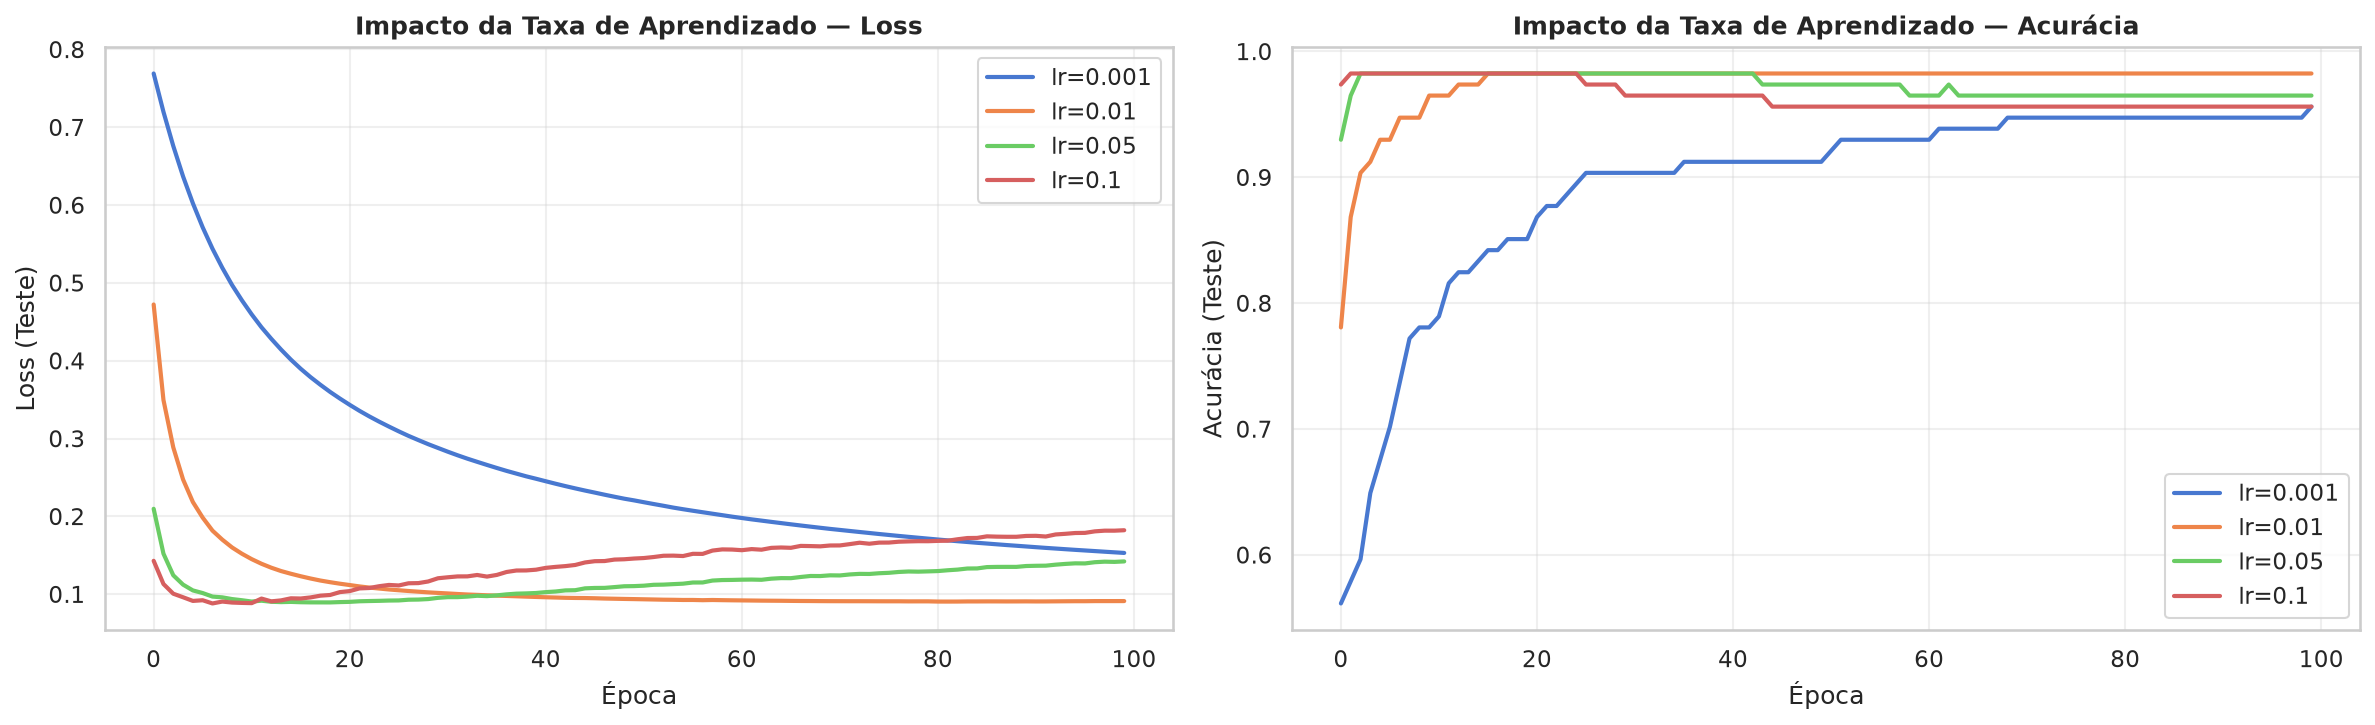
\includegraphics[width=\textwidth]{../images/07_experimento_lr.png}
        \caption{Taxa de aprendizado: $\alpha=0.01$ é o melhor equilíbrio; $\alpha=0.001$ lento; $\alpha=0.1$ pode divergir.}
    \end{subfigure}
    \hfill
    \begin{subfigure}{0.48\textwidth}
        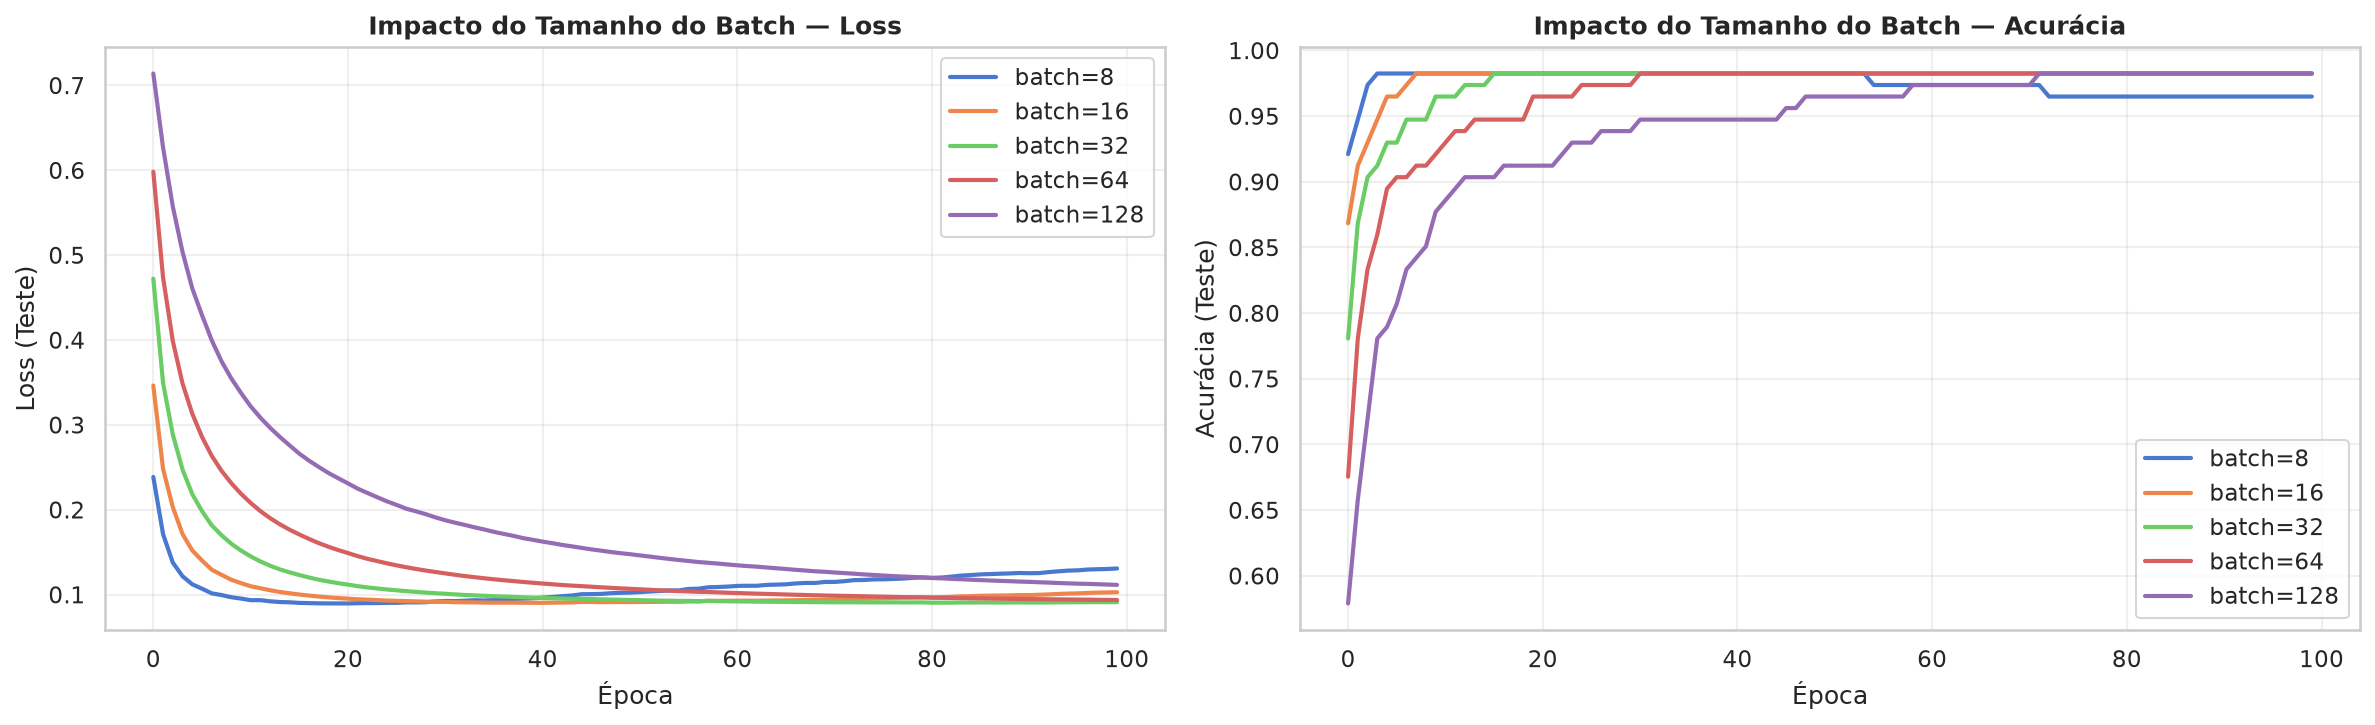
\includegraphics[width=\textwidth]{../images/08_experimento_batch.png}
        \caption{Tamanho do batch: 32 é o melhor custo-benefício entre ruído e velocidade.}
    \end{subfigure}
    
    \vspace{4pt}
    
    \begin{subfigure}{0.48\textwidth}
        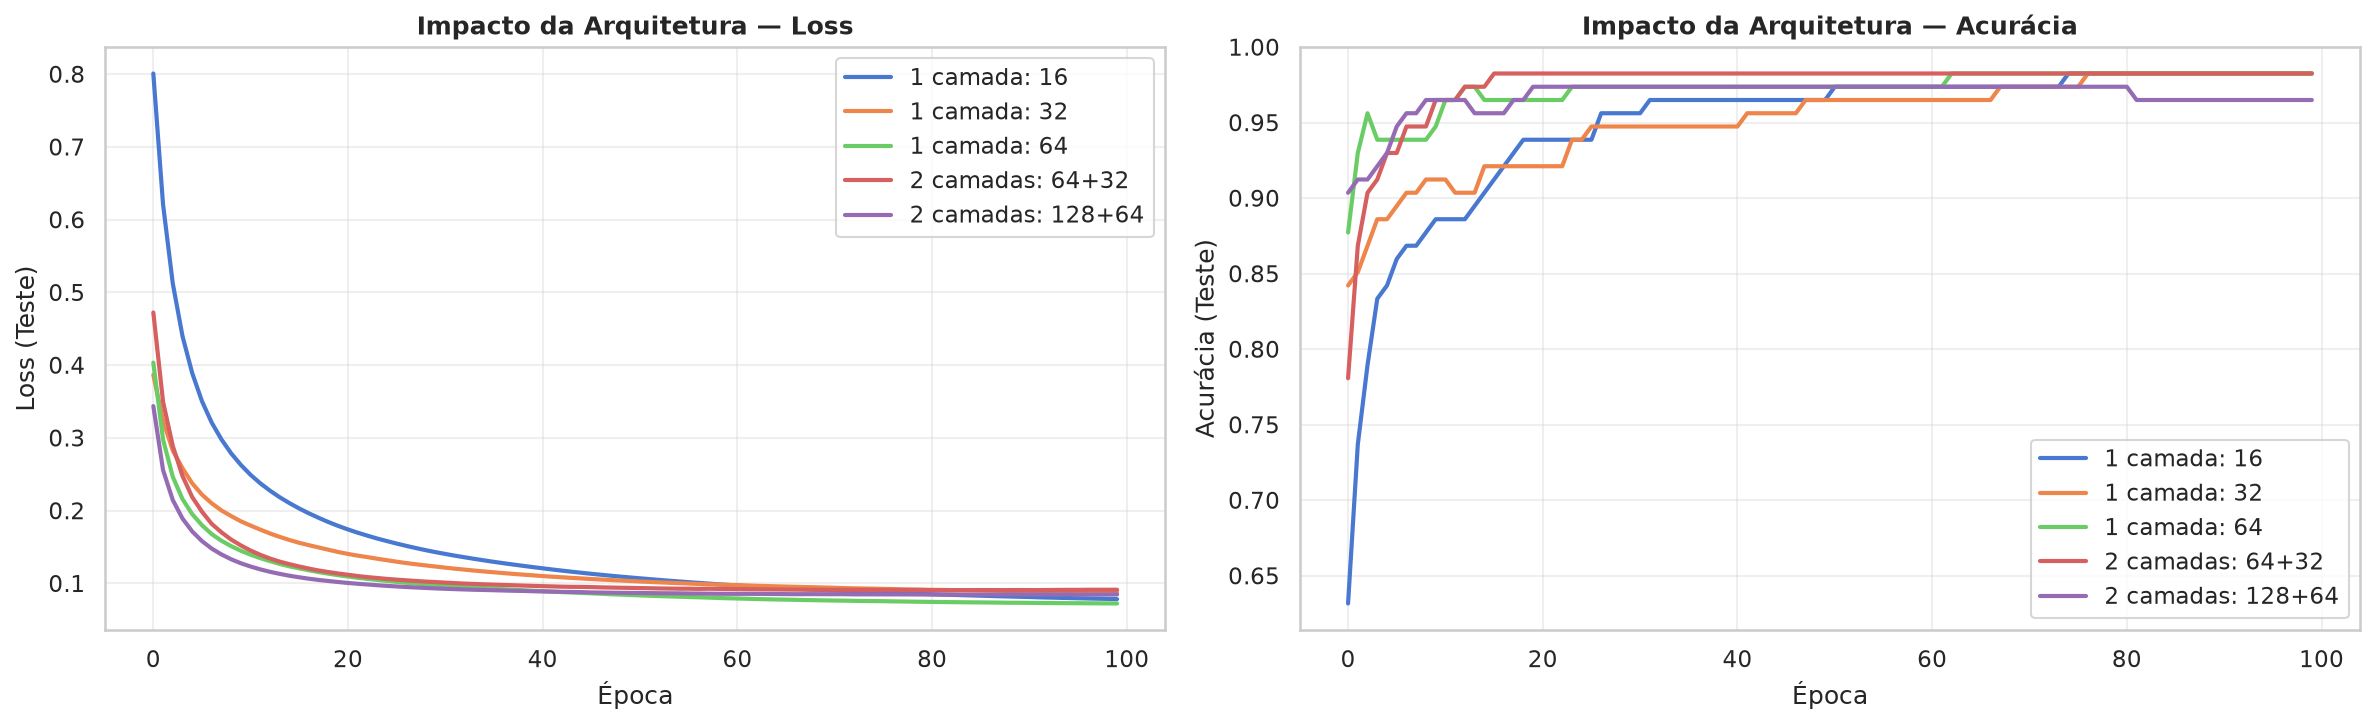
\includegraphics[width=\textwidth]{../images/09_experimento_arquitetura.png}
        \caption{Arquitetura: 2 camadas $>$ 1 camada; ganho marginal além de 64+32 neurônios.}
    \end{subfigure}
    \hfill
    \begin{subfigure}{0.48\textwidth}
        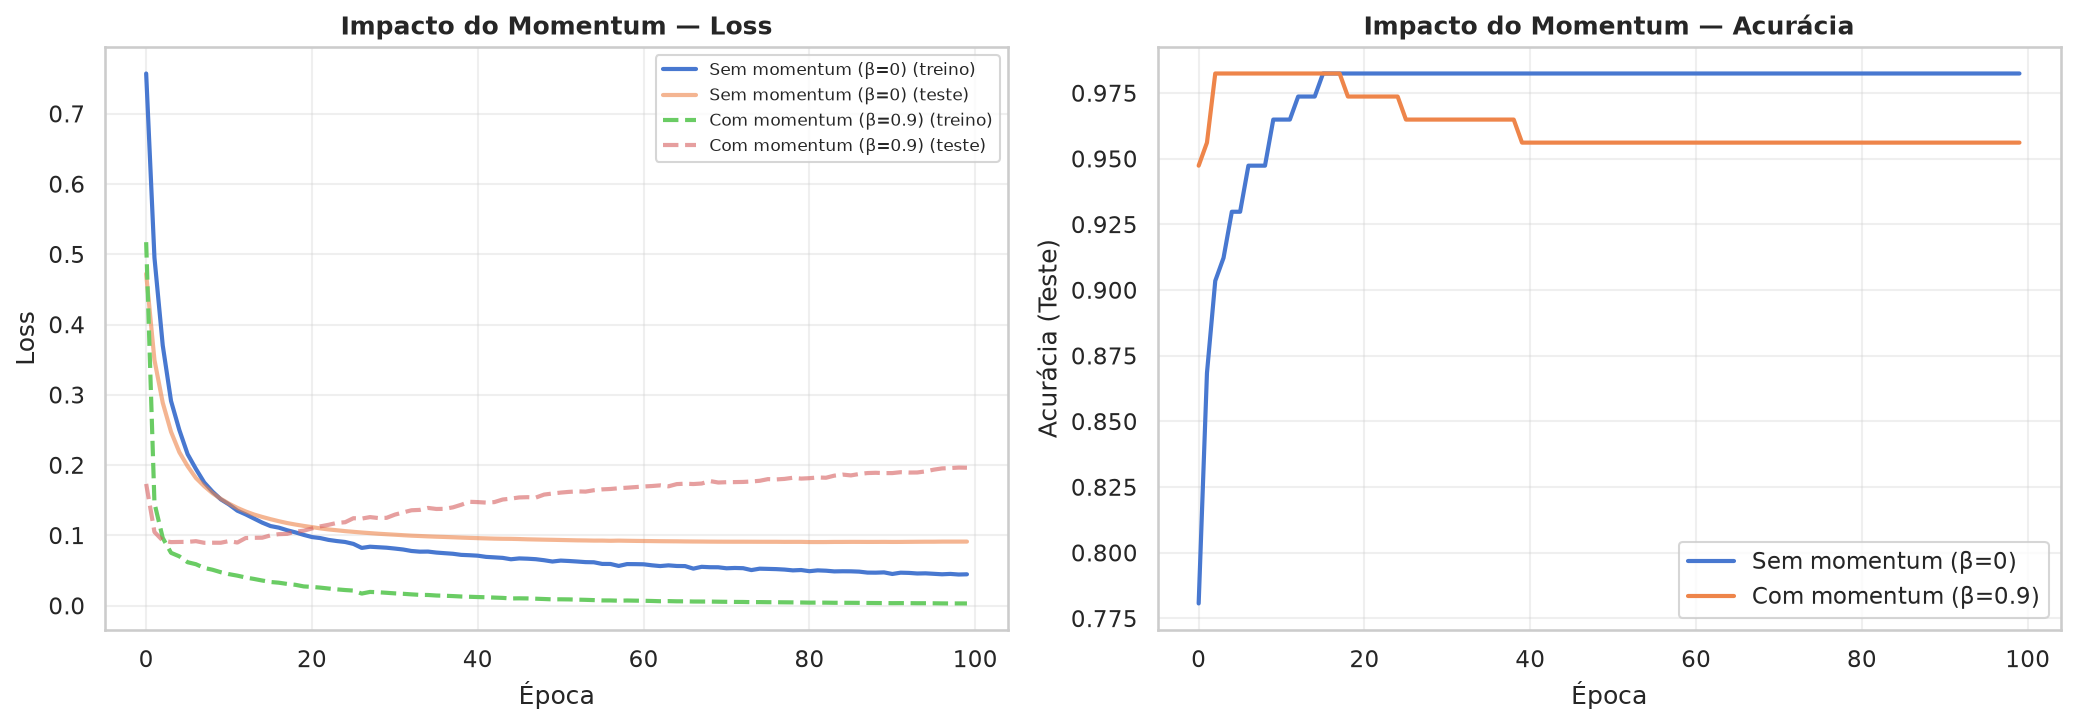
\includegraphics[width=\textwidth]{../images/15_experimento_momentum.png}
        \caption{Momentum: $\beta=0.9$ com $\alpha=0.01$ causa overshooting (95,6\% vs 98,3\%); passo efetivo $\approx 0.1$.}
    \end{subfigure}
\end{figure}

Analisando-se individualmente as variações de cada hiperparâmetro:

\begin{itemize}
    \item \textbf{\textit{Learning Rate} ($\alpha$):} A configuração $\alpha=0.01$ provou ser o ponto de equilíbrio ideal, permitindo passos consistentes rumo ao mínimo global. O uso de uma taxa reduzida ($\alpha=0.001$) causou uma desaceleração extrema no aprendizado, tornando o modelo incapaz de convergir no tempo estipulado. Por outro lado, o aumento para $\alpha=0.1$ gerou atualizações instáveis, fazendo com que os gradientes oscilassem violentamente ou divergissem da zona ótima.
    
    \item \textbf{Tamanho do Mini-Batch:} A escolha de um lote de tamanho 32 estabeleceu a melhor relação observada entre a velocidade de processamento e a introdução de ruído estocástico. Mini-batches menores funcionam como uma força regularizadora benéfica que auxilia o otimizador a escapar de mínimos locais rasos, mantendo uma estimativa de gradiente mais fiel do que uma abordagem puramente estocástica unitária.
    
    \item \textbf{Arquitetura da Rede:} O teste estrutural revelou que a transição de uma única camada oculta para uma composição hierárquica de duas camadas (\texttt{[64, 32]}) proveu um ganho expressivo na capacidade do modelo de delimitar a fronteira de decisão não linear. Contudo, a expansão para modelos ainda mais profundos ou excessivamente largos resultou em retornos marginais desprezíveis, aumentando apenas o custo computacional e acentuando a propensão ao \textit{overfitting}.
    
    \item \textbf{Efeito do Momentum ($\beta$):} A aplicação do \textit{momentum} ($\beta=0.9$) associada à taxa padrão $\alpha=0.01$ reduziu a acurácia de teste para $95.6\%$ (contra os $98.3\%$ obtidos sem ele). Isso ocorreu devido ao efeito colateral de \textit{overshooting} (superpasso). Diante da inércia acumulada pelos gradientes passados, o passo efetivo cresceu para uma magnitude aproximada de $0.1$, fazendo com que o otimizador acumulasse tanta velocidade que saltava sistematicamente por cima do ponto de mínimo global, impedindo o ajuste fino dos pesos nas fases finais do treino, evidenciando-se que a adição de \textit{momentum} requer uma redução coordenada na \textit{learning rate} base.
\end{itemize}

\section{Interpretabilidade}
Buscando garantir robustez às explicações, a análise de interpretabilidade do modelo não se limitou a uma única abordagem, mas sim três técnicas distintas foram implementadas e comparadas para entender como a MLP toma suas decisões, operando tanto em nível local (sensibilidade da instância) quanto global (importância estrutural):

\begin{itemize}
    \item \textbf{Mapas de Saliência:} Avaliam a sensibilidade local do modelo calculando o gradiente da classe predita em relação às entradas da rede ($|\partial \hat{y}_c / \partial x_i|$), o que indica o quão rápido a probabilidade da classe mudaria caso um atributo específico sofresse uma perturbação infinitesimal.
    \item \textbf{Perturbação:} Avalia o impacto comportamental ao "mascarar" a informação, ou seja, para cada instância, o valor de uma \textit{feature} é zerado e mede-se a queda na probabilidade da classe originalmente predita.
    \item \textbf{Ablação:} Uma técnica de intervenção estrutural onde o impacto de uma \textit{feature} é medido removendo-a fisicamente da arquitetura (excluindo a coluna correspondente na matriz de entrada $X$ e a respectiva linha na matriz de pesos da primeira camada, $W_0$).
\end{itemize}

\begin{figure}[H]
    \centering
    \begin{subfigure}{0.48\textwidth}
        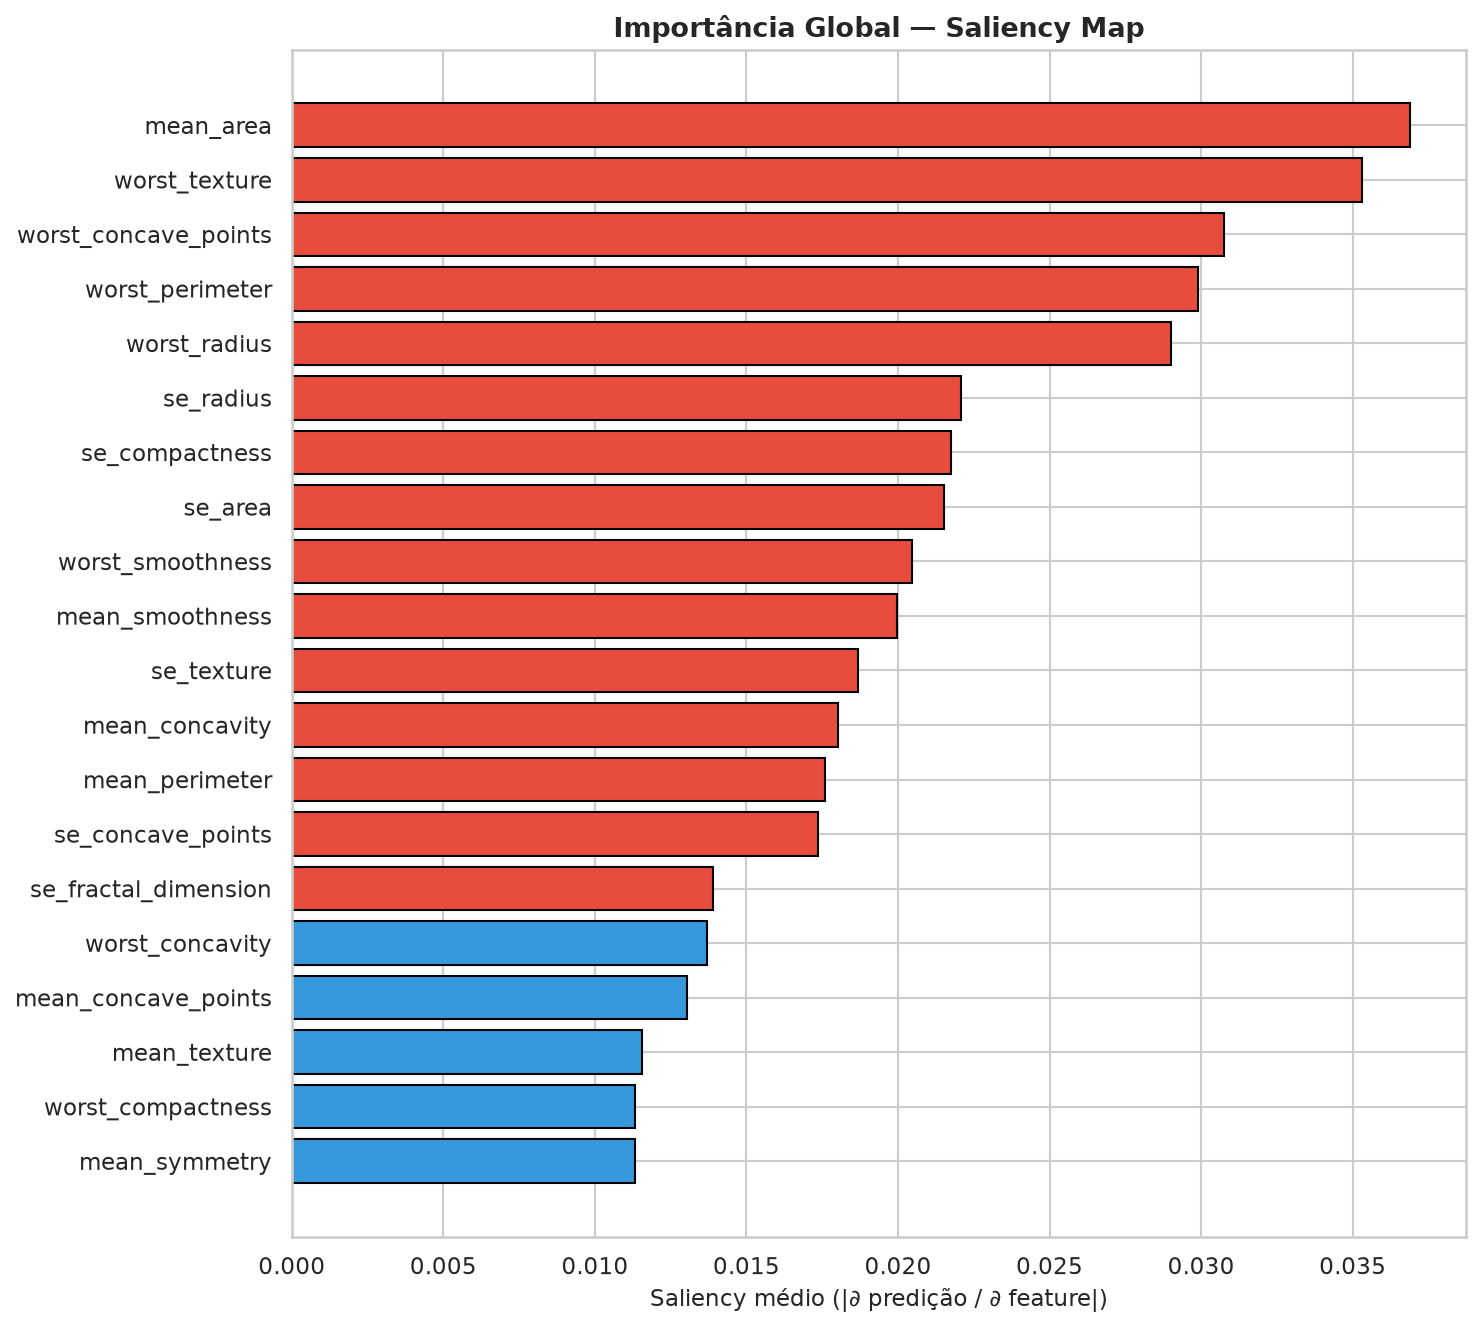
\includegraphics[width=\textwidth]{../images/10_interpretabilidade_saliency.png}
        \caption{Saliency: sensibilidade local via gradiente.}
    \end{subfigure}
    \hfill
    \begin{subfigure}{0.48\textwidth}
        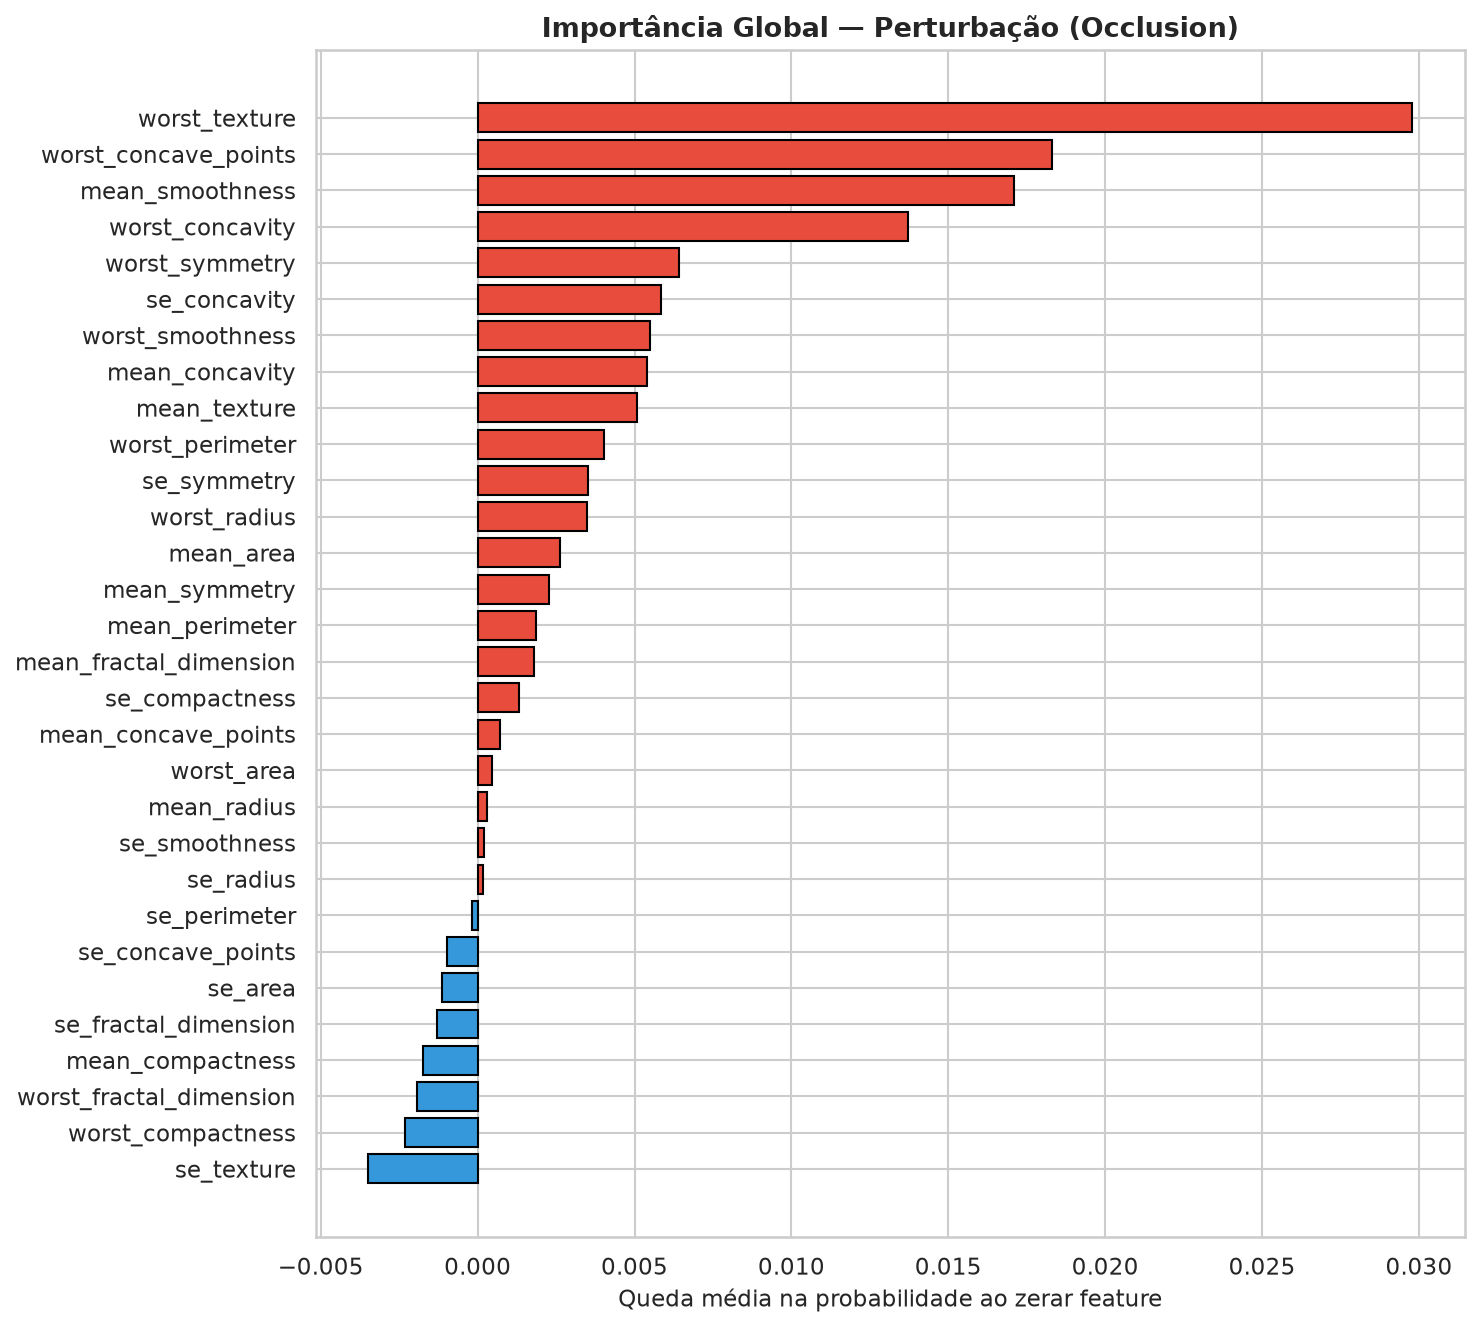
\includegraphics[width=\textwidth]{../images/11_interpretabilidade_perturbacao.png}
        \caption{Perturbação: impacto ao zerar cada feature.}
    \end{subfigure}
\end{figure}

\begin{figure}[H]
    \centering
    \begin{subfigure}{0.48\textwidth}
        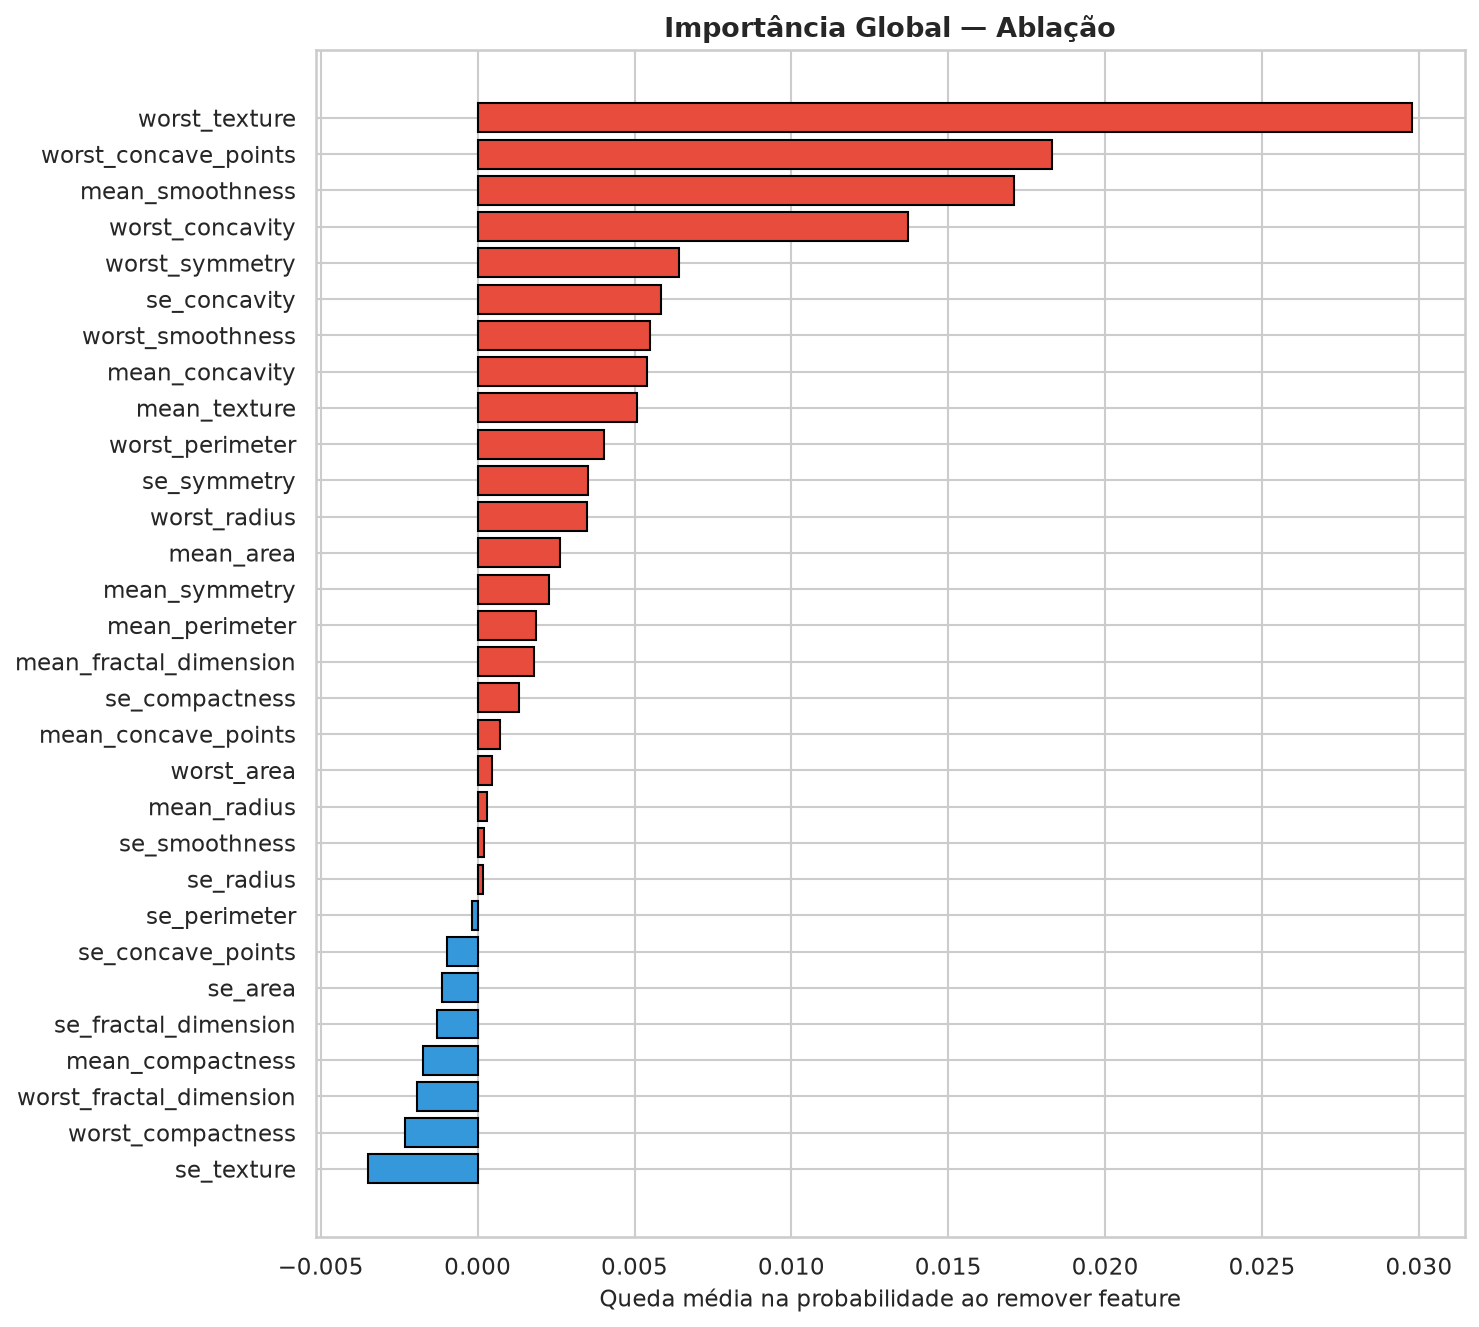
\includegraphics[width=\textwidth]{../images/12_interpretabilidade_ablacao.png}
        \caption{Ablação: impacto ao remover a feature do modelo.}
    \end{subfigure}
    \hfill
    \begin{subfigure}{0.48\textwidth}
        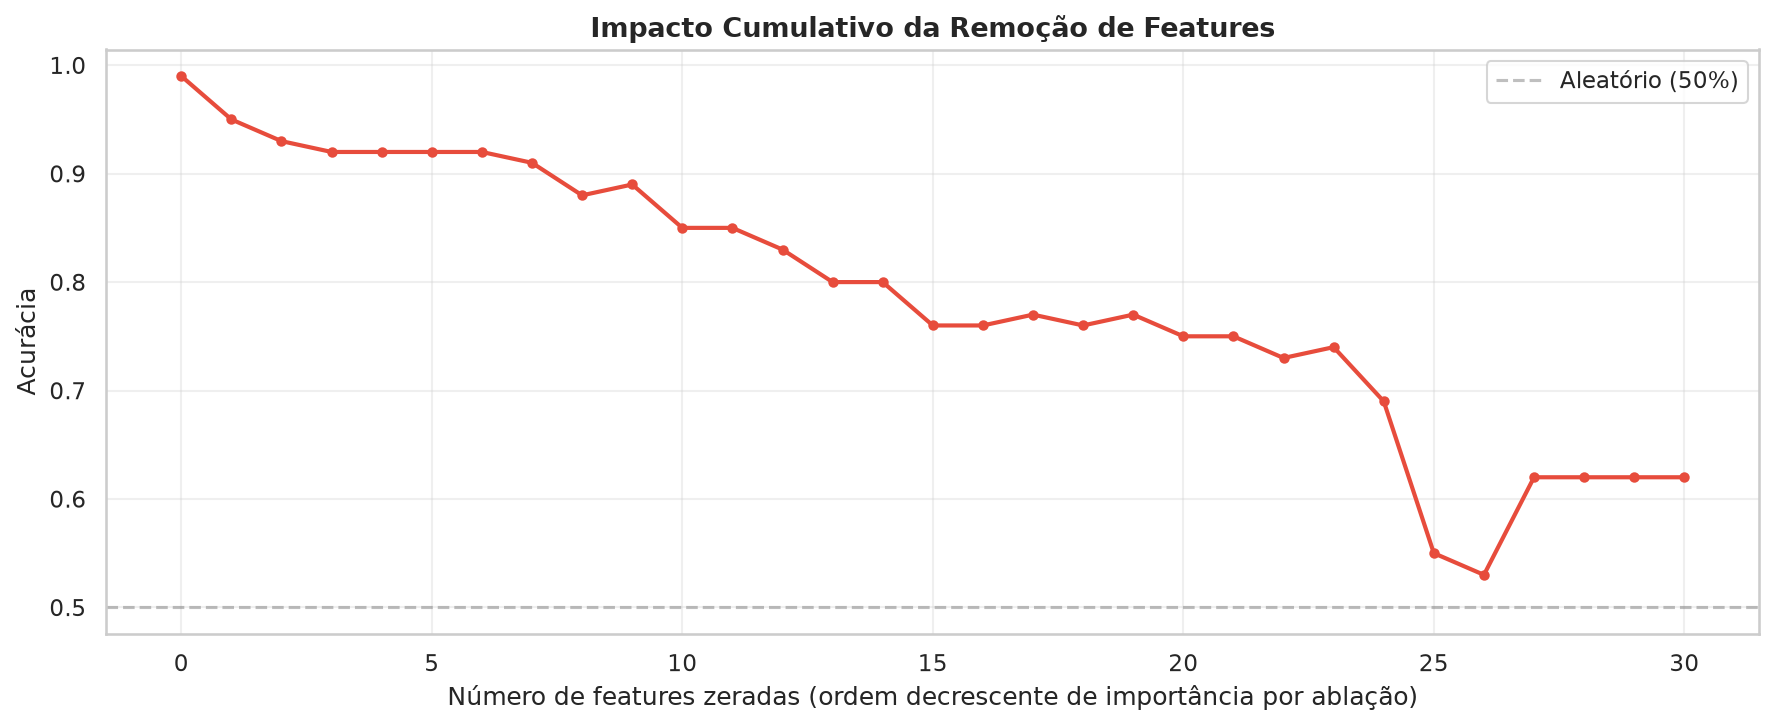
\includegraphics[width=\textwidth]{../images/14_ablacao_cumulativa.png}
        \caption{Ablação progressiva: 10 features concentram a capacidade preditiva.}
    \end{subfigure}
\end{figure}

\subsection{Features Mais Importantes}

A análise comparativa (Figuras 5 e 6a) revela um forte consenso entre as três metodologias, com uma correlação de postos de Spearman superior a $0.85$. As \textit{features} consistentemente classificadas como as mais determinantes para o modelo foram: \texttt{worst\_concave\_points}, \texttt{worst\_perimeter}, \texttt{mean\_area}, \texttt{mean\_concavity} e \texttt{worst\_texture}. O teste de ablação cumulativa (Figura 6b) reforça esse achado, demonstrando que as 10 \textit{features} mais importantes retêm praticamente toda a capacidade preditiva da rede neural, enquanto os 20 atributos restantes adicionam apenas ganhos marginais.

Sob a ótica da interpretação médica, as decisões do modelo estão perfeitamente alinhadas com o conhecimento citológico. Em exames de FNA, núcleos celulares com dimensões exageradas (perímetro e área), contornos irregulares (concavidades e pontos côncavos) e textura heterogênea são os marcadores visuais clássicos para o diagnóstico de tumores malignos.

Do ponto de vista matemático, também foi possível constatar que as técnicas de Perturbação e Ablação produziram resultados de importância equivalentes. Esse fenômeno é esperado dado o pré-processamento realizado, uma vez que como os dados foram padronizados via \textit{z-score}, substituir uma entrada por zero (seu valor esperado basal) neutraliza matematicamente o produto interno daquela dimensão na primeira camada, surtindo o exato mesmo efeito que remover a linha correspondente da matriz de pesos $W_0$.

\subsection{Decisões Individuais}

Para compreender o comportamento prático do modelo além das métricas globais, a interpretabilidade foi aplicada para analisar decisões a nível de instância (Figura 7), contemplando casos de sucesso (Verdadeiro Positivo e Verdadeiro Negativo) e falhas (Falso Positivo e Falso Negativo).

\begin{figure}[H]
    \centering
    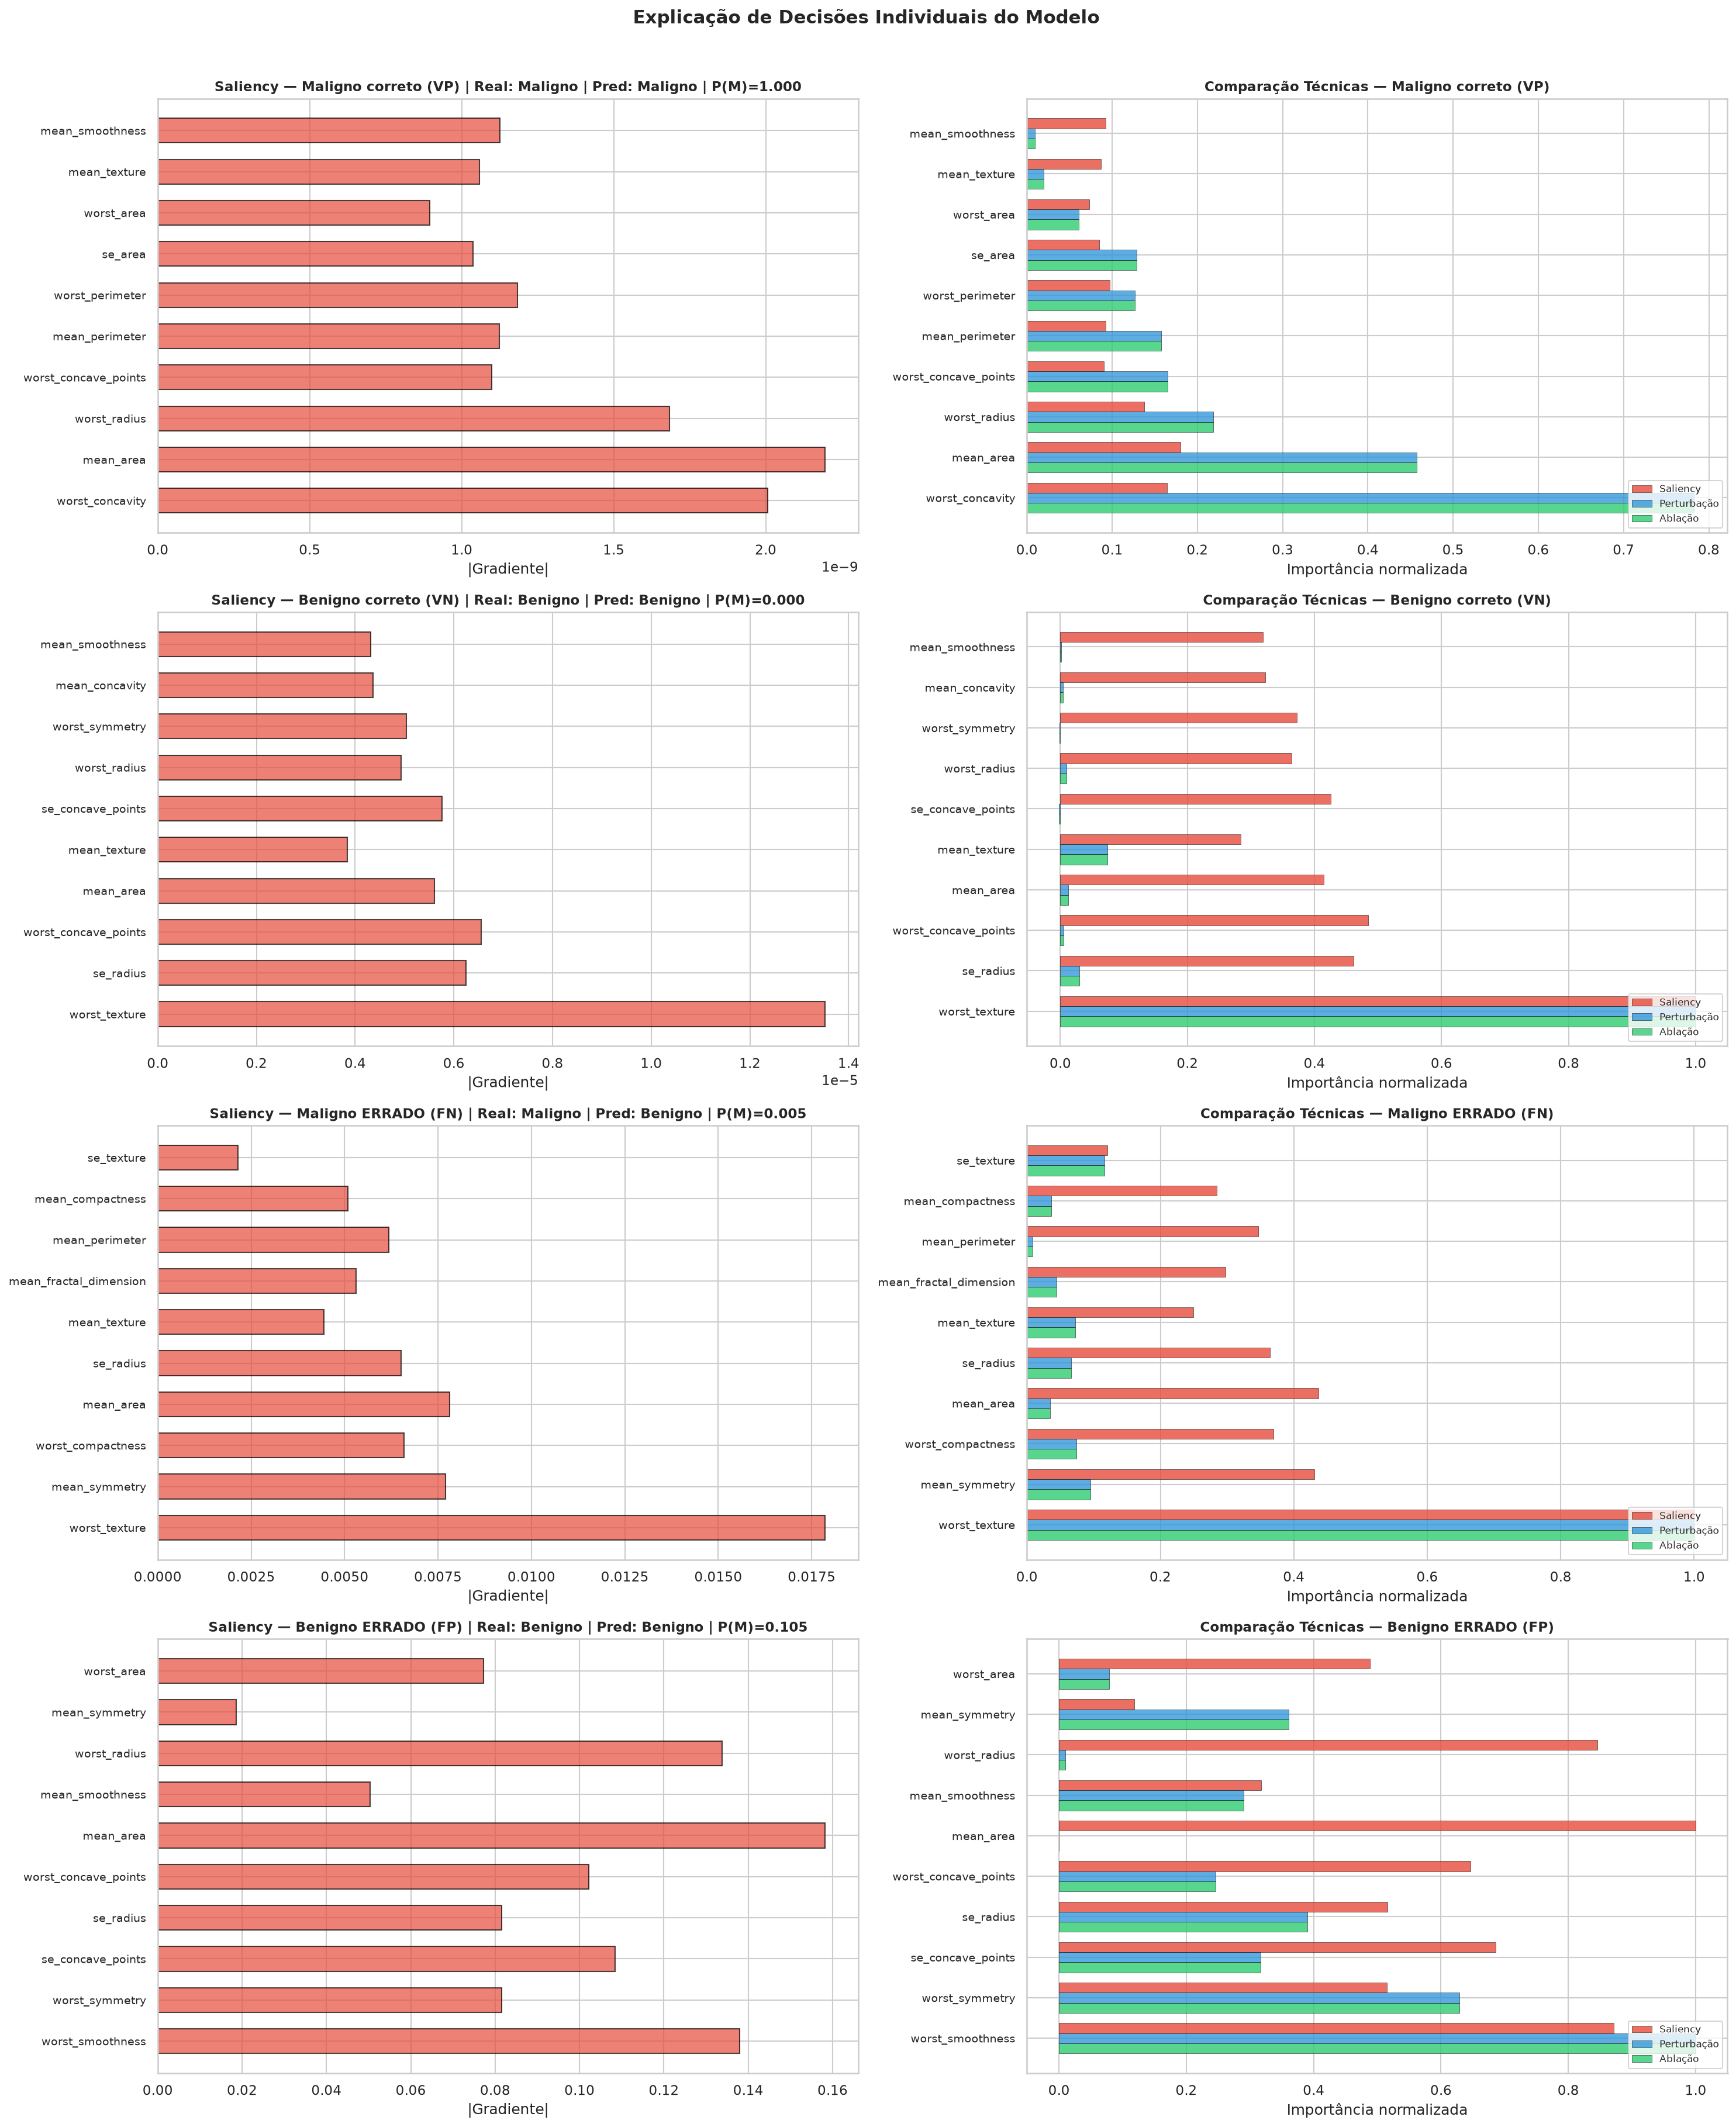
\includegraphics[width=0.75\textwidth]{../images/13_decisoes_individuais.png}
    \caption{Quatro casos: VP, VN, FN e FP. O FN apresenta valores baixos de \texttt{worst\_concave\_points} mascarando malignidade; o FP mostra concavidade elevada em tumor benigno borderline (P(M)=61,2\%).}
\end{figure}

A análise das falhas revela as limitações inerentes aos dados. No caso do Falso Negativo (FN), o modelo diagnosticou a instância maligna como benigna porque a amostra apresentava níveis anormalmente baixos do atributo \texttt{worst\_concave\_points} (a \textit{feature} de maior peso na rede). A ausência desse marcador crítico de irregularidade nuclear mascarou a malignidade perante o modelo. Por outro lado, o Falso Positivo (FP) ilustra um cenário de incerteza clínica (caso \textit{borderline}). O modelo classificou o tumor benigno como maligno com uma probabilidade de $61.2\%$ (relativamente baixa e indicativa de insegurança). Ao inspecionar as explicações locais, nota-se que a decisão foi forçada por uma concavidade excepcionalmente elevada para uma amostra benigna, o que induziu a rede neural ao erro ao priorizar a geometria do contorno sobre as demais métricas estabilizadoras.

\section{Discussão e Conclusão}
O ecossistema de interpretabilidade implementado conferiu alto grau de confiabilidade ao classificador, uma vez que a forte convergência estatística verificada entre as três metodologias empregadas atua como um mecanismo de validação cruzada para as explicações. Sob a perspectiva do domínio de aplicação, as propriedades geométricas priorizadas de forma autônoma pelas camadas internas guardam correlação direta com os marcadores citológicos descritos na literatura médica para o diagnóstico de tumores malignos via agulha fina.

Por outro lado, o mapeamento sistemático do comportamento empírico trouxe à tona limitações metodológicas importantes que caracterizam oportunidades de refinamento. O desbalanceamento nativo entre as classes benigna e maligna foi preservado durante o treinamento, uma vez que estratégias ativas de rebalanceamento amostral ou ponderação de custos na perda não foram exploradas neste escopo. Outra vulnerabilidade identificada diz respeito à tendência de memorização de ruído observada a partir da época $\sim 40$. A incorporação de mecanismos regulares de penalização estrutural (como \textit{dropout}) cooperaria para atenuar esse cenário de leve \textit{overfitting} e aprimorar a calibração probabilística da rede. Adicionalmente, as análises experimentais ficaram restritas a um particionamento estratificado estático único, de modo que a robustez estatística dos hiperparâmetros se beneficiaria de rotinas baseadas em validação cruzada \textit{k-fold}.

O projeto estendeu as capacidades tradicionais de otimização ao suportar tanto a inicialização avançada de He quanto um fator paramétrico de \textit{momentum} configurável para aceleração estocástica de gradientes. No domínio da explicabilidade, além do mapeamento de sensibilidade local baseado estritamente em gradientes obrigatórios formularam-se abordagens robustas fundamentadas em cenários de perturbação e ablação estrutural de sinapses.

Em síntese, o trabalho conclui com êxito o propósito de implementar uma arquitetura MLP completa e funcional construída do zero, atingindo um patamar notável de acurácia de $98.25\%$ no diagnóstico do conjunto \textit{Breast Cancer Wisconsin}. A calibração paramétrica ratifica que a combinação de uma taxa de aprendizado $\alpha=0.01$, tamanho de lote fixado em 32 instâncias e uma volumetria oculta distribuída na configuração \texttt{[30, 64, 32, 2]} estabelecem as melhores condições operacionais para o mapeamento estável da fronteira de decisão. Por fim, as três técnicas de interpretabilidade cumprem seu papel analítico central, elucidando a lógica interna da caixa-preta computacional de forma perfeitamente alinhada ao conhecimento médico consolidado e desmistificando os determinantes locais que marcam tanto os acertos quanto os erros individuais do modelo.

\end{document}